\documentclass[11pt,a4paper]{article}

\usepackage[T1]{fontenc}
\usepackage[utf8]{inputenc}
\usepackage{newunicodechar}
\newunicodechar{ℝ}{\ensuremath{\mathbb{R}}}
\newunicodechar{∀}{\ensuremath{\forall}}
\newunicodechar{∃}{\ensuremath{\exists}}
\newunicodechar{≠}{\ensuremath{\neq}}
\newunicodechar{→}{\ensuremath{\to}}
\usepackage{mathptmx}
\usepackage[expansion=false]{microtype}
\usepackage[margin=2.6cm]{geometry}
\usepackage{amsmath,amssymb,amsthm,mathtools}
\usepackage{booktabs,tabularx,array}
\usepackage{enumitem}
\usepackage{xcolor}
\usepackage[most]{tcolorbox}
\usepackage{pgfplots}
\pgfplotsset{compat=1.16}
\usetikzlibrary{positioning,arrows.meta,fit,calc,backgrounds}
\usepackage[authoryear,round]{natbib}
\usepackage[colorlinks=true,linkcolor=blue!55!black,citecolor=blue!55!black,urlcolor=blue!55!black]{hyperref}

\setlist{itemsep=2pt,topsep=3pt,parsep=0pt}
\setlength{\emergencystretch}{3em}
\setlength{\parskip}{3pt}
\renewcommand{\arraystretch}{1.15}
\bibliographystyle{plainnat}

% ---------- theorem environments (one shared counter, numbered by section)
\theoremstyle{plain}
\newtheorem{theorem}{Theorem}[section]
\newtheorem{proposition}[theorem]{Proposition}
\newtheorem{lemma}[theorem]{Lemma}
\newtheorem{corollary}[theorem]{Corollary}
\theoremstyle{definition}
\newtheorem{definition}[theorem]{Definition}
\newtheorem{axiom}[theorem]{Axiom}
\newtheorem{example}[theorem]{Example}
\theoremstyle{remark}
\newtheorem{remark}[theorem]{Remark}

% ---------- purpose line printed above every formal statement
\newcommand{\purpose}[1]{\par\smallskip\noindent{\small\upshape\leftskip=1.1em\rightskip=1.1em
  \textsc{Purpose.}\ #1\par}\vspace{-1pt}}

% ---------- notation
\newcommand{\R}{\mathbb R}
\newcommand{\E}{\mathbb E}
\newcommand{\LR}{\mathrm{LR}}
\newcommand{\Rext}{\widehat{\mathbb R}_\star}
\newcommand{\1}{\mathbf 1}
\newcommand{\TV}{\mathrm{TV}}
\newcommand{\ess}{\operatorname{ess\,sup}}
\newcommand{\eqd}{\overset{d}{=}}
\newcommand{\Hset}{\mathcal H}
\newcommand{\Xp}{\mathcal X}
\newcommand{\ax}[1]{\textup{(\textsf{#1})}}
\newcommand{\axCP}{\ax{CP}}
\newcommand{\axLI}{\ax{LI}}
\newcommand{\axCM}{\ax{CM}}
\newcommand{\axRC}{\ax{RC}}
\newcommand{\axRM}{\ax{RM}}
\newcommand{\bracket}[2]{[#1\!:\!#2]}

\newtcolorbox{keybox}[1][]{colback=blue!4!white,colframe=blue!45!black,
  boxrule=0.5pt,arc=2pt,left=6pt,right=6pt,top=4pt,bottom=4pt,breakable,#1}

\newcommand{\axP}{\ax{P}}
\newcommand{\axN}{\ax{N}}

\title{\textbf{An Axiomatic Characterization of the Loss Ratio}}
\author{Hirbod Assa\thanks{Climate Parametric Risk Solutions and University College Dublin.
  \emph{Draft of 25 October 2026.} The use of generative AI in this work is described in Section~\ref{sec:collab}
  and in the declaration before the references. The proofs have undergone AI-assisted critical review, which is
  fallible and does not constitute formal verification; the loss-ratio-specific steps have in addition been
  checked in Lean in an abstract setting. See Section~\ref{sec:collab-status}.}}
\date{}

\begin{document}
\maketitle

\begin{abstract}
\noindent
This paper has a twofold aim: to introduce and study in depth the loss ratio, a concept of central practical
importance in actuarial science, and to provide a case study of how generative AI can support mathematical work in
actuarial mathematics under close human supervision. The loss ratio $\LR(X)$ of an insurance book $X$ is
the ratio of a loss measure $\rho(X)$ to a premium $\Pi(X)$, yet it has no axiomatic theory of its own. We show that
both parts can be \emph{implied} by the loss ratio itself. Along the cash line $c\mapsto\LR(X+c)$, obtained by adding
sure losses $c$ to the book, there is exactly one point where the ratio stops being finite; its location is the
\emph{implied premium}, the sure payment at which the book changes hands. The \emph{implied risk measure}
then follows from the accounting identity loss $=$ loss ratio $\times$ premium, and it is visible even where the
ratio explodes, as the residue of the singularity. With this reading, four natural axioms on the loss ratio --
a single non-finite point on each cash line, a loss ratio of one for sure losses, premium-weighted comonotone
pooling, and law invariance -- together with continuity (respectively monotonicity) of the implied premium and risk
measure characterize the loss ratios $\LR=I_h/I_g$, where $I_h,I_g$ are signed Choquet integrals with distortion
functions $h,g$ (respectively distortion premia), with $(h,g)$
unique. The unit-slope M\"obius form of the cash lines, comonotonic additivity of the implied premium, and
the association with a family of risk measures are derived rather than assumed. We show that no non-trivial loss ratio is monotone, show by
counterexamples that none of the axioms except the one defining the implied premium can be dropped, and state candidly which parts of the result are classical. The work used Claude (Anthropic) as a main
assistant and to run panels of AI agents that surveyed the literature, proposed and ranked candidate statements,
drafted proofs and counterexamples, and reviewed the proofs critically; ChatGPT and Gemini were used for an
informal review of the proofs and for summaries of cited works. All decisions on content were the author's, and
the AI output was treated as proposals: reviews found and corrected errors, and the steps specific to loss ratios
were formalized and checked in the proof assistant Lean, with the classical representation step as a hypothesis.
A final section reports this use, the errors found, the guardrails and the verification status.
\end{abstract}

\noindent\textbf{Keywords:} loss ratio; implied premium; implied risk measure; axiomatic characterization;
distortion premium; signed Choquet integral; comonotonic additivity.

\section{Introduction}\label{sec:intro}

The loss ratio, claims divided by premium, is among the most widely used quantities in insurance
underwriting, portfolio management and reinsurance pricing. Ex post it is incurred claims over earned
premium; ex ante it is the ratio of a loss measure $\rho(X)$, such as an expected or a risk-adjusted loss, to a
premium $\Pi(X)$ of the same position $X$. When the premium is a non-linear functional of the loss, or the
numerator is a risk measure, it is not clear which functionals of a loss should be called a loss ratio, or
which properties a loss ratio should have when books are pooled.

The question arises in risk reporting. Before the claims are known, a loss ratio is usually reported through
its expected value, expected claims over premium. When the risk of a book is concentrated in the tail of its
loss distribution, the expected loss ratio can be misleading: two books with the same expected loss ratio may
differ greatly in their exposure to large losses. A natural remedy is to replace the mean of the claims by a tail
measure, and to report, for instance, the value at risk or the tail value at risk (expected shortfall) of the claims divided by the
premium \citep{adeh1999}. The loss ratio then becomes a model-based, or mark-to-model, quantity: a risk measure
of the loss, evaluated under a model of its distribution, divided by a premium principle. The ex-post accounting
ratio is the special case in which the model is the realized outcome. Once such ratios are admitted, the
question is which properties are necessary and sufficient for a functional of the loss to be a loss ratio of
this kind; this is the question addressed here. The tail value at risk and the value at risk are distortion
functionals, so tail loss ratios over a distortion premium are covered by the results below
(see the ratio $\mathrm{ES}_{0.9}/\E$ in Example~\ref{ex:qc}).

We work with the \emph{extended loss ratio} $\LR=\rho/\Pi$, which allows negative values and zero premiums,
defined abstractly by \emph{association}: a family of risk measures $\{\rho_\beta\}$ is
associated with $\LR$ if $\LR(X)=\beta\iff\rho_\beta(X)=0$; the canonical family is
$\rho_\beta=(\rho-\beta\Pi)/(1-\beta)$, $\beta\ne1$. The present paper characterizes, by axioms stated on $\LR$
alone, the loss ratios that are ratios of two Choquet-type functionals.

Three features distinguish the problem from the classical characterizations of premium principles and risk
measures \citep{yaari1987,wyp1997,schmeidler1986,www2020}. First, the object is a ratio, while those results
concern a single functional. Second, the ratio does not determine its numerator and denominator: on positive
losses, $(\rho,\Pi)$ and $(\psi\rho,\psi\Pi)$ give the same ratio for every positive functional $\psi$. Third, the
ratio is not monotone: we show that a loss ratio of two distortion functionals is monotone only if it is
identically $1$ (Proposition~\ref{prop:F2}), so the theory of acceptability indices, which rests on monotonicity
\citep{chernymadan2009}, does not apply.

Our approach is to recover the premium and the risk measure from the loss ratio. For a book $X$, consider the
\emph{cash line} $c\mapsto\LR(X+c)$. A premium is the sure amount at which a risk changes hands; on the cash line,
a zero premium is a point at which the loss ratio is not finite. We define the \emph{implied premium} $\Pi(X)$ as
minus the unique such point, and the \emph{implied risk measure} by the accounting identity
$\rho(X)=\Pi(X)\LR(X)$, extended by cash shifts to books with zero premium. At such books the implied risk
measure is the residue of the cash line at its singularity (Proposition~\ref{prop:readings}). For a Bernoulli loss
$\1_A$ with $P(A)=\tfrac14$, the expected loss and the square-root distortion premium, the cash line is
$(\tfrac14+c)/(\tfrac12+c)$; it is singular at $c=-\tfrac12$, so $\Pi(\1_A)=\tfrac12$ and
$\rho(\1_A)=\tfrac12\LR(\1_A)=\tfrac14$ (Figure~\ref{fig:three}).

With this reading, Theorems~\ref{thm:A} and~\ref{thm:B} state the following. A map $\LR$ from bounded losses to
$\R\cup\{\infty,\star\}$ is of the form $I_h/I_g$, with $I_h,I_g$ signed Choquet integrals of distortions $h,g$
of bounded variation, if and only if it satisfies the following axioms, stated in Section~\ref{sec:axioms}:
\axP{} every cash line has exactly one point where $\LR$ is not finite; \axN{} $\LR(c)=1$ for sure losses
$c\ne0$; \axCM{} the loss ratio of a pool of comonotone books is a combination of their loss ratios with their relative costs, $\Pi(X)/(\Pi(X)+\Pi(Y))$, as weights; \axLI{} $\LR$ is
law invariant; and \axRC{} the implied premium and risk measure are uniformly continuous. If \axRC{} is replaced
by \axRM, monotonicity of the implied premium and risk measure, $h$ and $g$ are distortion functions and no continuity
assumption is needed. In both cases $(h,g)$ is unique, $\Pi=I_g$ and $\rho=I_h$. The unit-slope Möbius form of the
cash lines, the normalization $\Pi(c)=c$, comonotonic additivity of the implied premium, scale invariance and
the association are consequences of the axioms.

Given \axP{} and \axN, axiom \axCM{} is equivalent to comonotonic additivity of the implied premium and risk measure,
the axiom of \citet{yaari1987} and \citet{wyp1997}; once this equivalence is established, the representation step
follows from the theory of comonotonic additive functionals \citep{schmeidler1986,msm1994,cmmm2012,www2020}. The
contributions specific to loss ratios are: the construction of the implied premium and risk measure; the proof
that the pooling identity yields additivity of the implied pair on all comonotone pairs, including books that
break even, on which a premium given exogenously would not be identified (Lemma~\ref{lem:comon} and
Remark~\ref{rem:primitive}); unconditional uniqueness of $(h,g)$; the impossibility of a monotone loss ratio and
its consequences for the associated family (Corollary~\ref{cor:assoc}); a version for nonnegative losses
(Theorem~\ref{thm:C}); and counterexamples showing that none of the axioms
\axN, \axCM, \axLI, \axRC, \axRM{} can be dropped.

The paper has a second aim: it is a brief case study of the use of AI in mathematical research in actuarial
science. The work was done with Claude (Anthropic), used as a main assistant and to coordinate panels of AI
agents on designated parts of the project: a roundtable of six agents and a larger panel covering ten literature
strands surveyed the literature, proposed candidate statements, ranked them by judge agents, drafted proofs and
submitted them to repeated AI-assisted critical review; the main assistant constructed examples and
counterexamples and drafted and revised the manuscript. ChatGPT (OpenAI) was used for an informal review of the
proofs, and Gemini (Google) for summaries of key cited works. The problem was chosen by the author, from the
risk-reporting question above, and in part as a deliberate test: its solution requires machinery, such as
signed Choquet integrals, that is not routine, which makes it a demanding case for AI assistance. The research questions and all decisions on content
were the author's, and the formulation through the implied premium and the implied risk measure arose from the
author's objections to earlier AI-drafted versions, in particular that an assumed cash-line axiom supplied $\rho$
and $\Pi$ by fiat. The AI-generated material was treated as proposals: the reviews found errors, including a
wrong sufficient condition for quasi-convexity and an incorrect uniqueness claim, which were corrected (Table~\ref{tab:errors}); the
numbers in the examples were recomputed; the statements taken from three of the main sources were checked against
those papers; and the steps specific to loss ratios were formalized in the proof assistant Lean and checked by its
kernel, with the classical representation step taken as a hypothesis. Section~\ref{sec:collab} describes this
process, the errors and guardrails, and what has not been verified, and illustrates a standard for reporting such
use in a mathematical paper.

The paper is organized as follows. Section~\ref{sec:lit} reviews the related literature, and
Section~\ref{sec:setting} introduces the extended loss ratio. Section~\ref{sec:axioms} defines the implied premium
and risk measure and states the axioms. Section~\ref{sec:results} contains the main theorems and examples, and
Section~\ref{sec:triviality} discusses the role of the axioms. Proofs are in Section~\ref{sec:proofs}.
Section~\ref{sec:actuarial} treats nonnegative losses, Section~\ref{sec:necessity} gives the counterexamples, and
Section~\ref{sec:consequences} derives consequences. Section~\ref{sec:discussion} lists open problems, and
Section~\ref{sec:collab} describes the use of AI, including the formal check in Lean
(Section~\ref{sec:collab-lean}).

\section{Related literature and what is different here}\label{sec:lit}

The loss ratio touches four literatures: the axiomatic theory of premia and risk measures, the
theory of performance ratios and acceptability indices, implicitly defined risk functionals, and
ratio representations in decision theory and statistics. For each we say what is known, what we use,
and where our problem differs. Section~\ref{sec:lit-table} collects the differences in a table.

\subsection{Distortion premia, Choquet integrals and signed Choquet integrals}

The axiomatic theory of insurance premia starts from properties of a single premium functional
$H$ on losses: translation invariance, $H(X+c)=H(X)+c$, and ``no unjustified loading'', $H(c)=c$ for constant
losses \citep{gerber1974},
monotonicity, law invariance, and, most importantly, additivity for comonotonic risks. The dual
theory of \citet{yaari1987} replaces utility transformations of payoffs by distortions of probabilities, which
leads to the Choquet-type representation $\int g(P(X>x))\,dx$ and to additivity for comonotonic risks, and \citet{wang1996} introduced it as a premium principle. \citet{wyp1997}
characterize the \emph{distortion premium} $C_g$ by law invariance, monotonicity, comonotonic
additivity, a continuity condition and $H(1)=1$. The mathematical backbone is Schmeidler's
(\citeyear{schmeidler1986}) theorem: a monotone, comonotonic additive functional on bounded
measurable functions is a Choquet integral with respect to a capacity, with no continuity needed;
see also \citet{greco1982} and \citet{denneberg1994} on cones. Coherent risk measures are defined by
monotonicity, translation invariance, subadditivity and positive homogeneity \citep{adeh1999,delbaen2002}; in the
law-invariant case, comonotonic coherent risk measures are mixtures of expected shortfalls over levels in $[0,1]$
\citep{kusuoka2001,jst2006,folmerschied2016}.

Without monotonicity the corresponding representation theory is that of \emph{signed} Choquet
integrals. \citet{msm1994} and \citet{cmmm2012,cmmm2015} show that comonotonic additive functionals
of bounded variation are exactly differences of Choquet integrals with respect to set functions of
bounded variation. \citet{www2020} prove the law-invariant version used here: on an atomless
$L^\infty$, a functional is law invariant, comonotonic additive and uniformly norm continuous if and
only if it is a signed Choquet integral $I_h$ with $h$ of bounded variation. They also show that
$I_h$ is convex if and only if $h$ is concave, and \citet{wangwei2020} study when level sets of such
functionals are convex. \citet{www2020b} extend the characterization to law-invariant convex cones containing
$L^\infty$, such as $L^p$, by adding continuity at infinity, which holds automatically on $L^\infty$, and give a
representation of convex signed Choquet integrals by mixtures of expected shortfalls.

These theorems underlie our representation step, and
Theorems~\ref{thm:A} and~\ref{thm:B} are the loss-ratio counterparts of \citet[Thm.~1]{www2020} and
of \citet{wyp1997}. We re-prove the representation directly (Steps~5--8 of Section~\ref{sec:proofs})
to keep track of constants and because we need no continuity in the monotone tier.

All of these results characterize one functional by axioms placed on that
functional. A loss ratio is a ratio of two, and the axioms must be placed on the ratio, which does
not determine its parts (Section~\ref{sec:intro}). Bridging this gap is the content of
Sections~\ref{sec:axioms} and~\ref{sec:proofs}. We are not aware of an if-and-only-if
characterization of a ratio of two Choquet integrals, or of two risk measures, in this literature.

\subsection{Performance ratios and acceptability indices}

The best-known ratios of risk functionals are performance measures. The gain--loss ratio of
\citet{bernardoledoit2000} divides the expected positive part of a payoff by the expected negative
part, and \citet{biaginipinar2013} study its optimization. \citet{chernymadan2009} give an
axiomatic theory of \emph{acceptability indices}: a map $\alpha$ that is monotone, quasi-concave,
scale invariant and Fatou is characterized by an increasing family of coherent risk measures
$\{\rho_x\}$ with $\alpha(X)=\sup\{x:\rho_x(X)\le0\}$, and the family is recovered by the cash-shift
formula $\rho_x(X)=\inf\{c:\alpha(X+c)\ge x\}$. Dynamic versions and the correspondence between
indices and families are developed by \citet{bcz2014} and \citet{bbn2014}, and the correspondence
between quasi-convex functionals and acceptance families by \citet{drapeaukupper2013}. The
Sharpe ratio is not an index in this sense, and the conic-finance programme of
\citet{chernymadan2010} uses the \emph{spread} between ask and bid prices instead of a ratio.
\citet{ck2013} propose reward--risk ratios, a reward functional divided by a risk functional, and
list axioms that make such a ratio a performance measure, giving sufficient conditions rather than a
characterization. 

\citet{hlw2025} give an axiomatic theory of diversification indices. They note that the diversification
ratio $\phi(\sum_iX_i)/\sum_i\phi(X_i)$ of a risk measure $\phi$ may be negative, needs the conventions $0/0=0$
and $1/0=\infty$, and is not location invariant, and they characterize instead the \emph{diversification
quotient} $\alpha^*/\alpha$, where $\alpha^*$ is the level at which a decreasing family $(\rho_\beta)$ of risk
measures, evaluated at the pooled portfolio, reaches $\sum_i\rho_\alpha(X_i)$. Six axioms (non-negativity,
location and scale invariance, rationality, normalization and continuity) characterize the quotients built from
monotone, cash-additive and positively homogeneous families \citep[Thm.~1]{hlw2025}, and portfolio convexity
restricts the class to coherent families when there are at least four assets \citep[Thm.~2]{hlw2025}; they also
relate the quotient to the acceptability indices of \citet{chernymadan2009}. This is the closest if-and-only-if
result of association type. It shares two features with ours: a ratio-type quantity is recovered as the level at
which a family of risk measures crosses a threshold (compare Corollary~\ref{cor:assoc}), and the naive ratio
needs conventions where its denominator vanishes (compare the labels $\infty$ and $\star$). It differs in the
object, an index on vectors of risks that is invariant under location and scale, whereas a loss ratio is a
function of a single book that moves along each cash line as a M\"obius map; and in monotonicity, which their
rationality axiom uses and which a loss ratio cannot have (Proposition~\ref{prop:F2}).

The cash-shift recovery formula of \citet{chernymadan2009} and its
generalizations is the model for our reading of $\rho$ and $\Pi$ from cash lines, and the association is the
loss-ratio analogue of the level-crossing definition of an index. Three differences matter.

First, \emph{direction}. In an acceptability index, larger gains are better, so
the index is monotone and the family $\{\rho_x\}$ is monotone in the level. In a reward--risk ratio,
the numerator is a reward and the denominator a risk, so the ratio is monotone again. In a loss
ratio, numerator and denominator are both increasing in the loss. We show that the ratio is then
not monotone (Proposition~\ref{prop:F2}), and that the associated family
$\rho_\beta=(\rho-\beta\Pi)/(1-\beta)$ is not monotone either (Corollary~\ref{cor:assoc}): it is a
\emph{signed} Choquet integral even when $\rho$ and $\Pi$ are distortion premia. The index theorems
therefore do not apply, and the signed tier of Theorem~\ref{thm:A} is not a luxury but the natural
home of the associated family. Second, \emph{cardinality}. Indices are ordinal objects, determined up to
increasing transformations, whereas the loss ratio is cardinal: it obeys an accounting identity
under pooling (Section~\ref{sec:cm}). Third, \emph{what is characterized}. We characterize
the ratio together with its numerator and denominator, not an index through a family.

\subsection{Level-crossing and implicitly defined functionals}

Several risk functionals are defined implicitly, by where a monotone family crosses a level. Orlicz
premia solve $\E[\varphi(X/\pi)]=1-\alpha$ for $\pi$ \citep{hg1982,brg2008}, and PELVE is the
level at which expected shortfall equals a given value-at-risk
\citep{liwang2023,fiorirg2023}. Return risk measures \citep{blrg2018} and star-shaped risk measures
\citep{castagnoli2022} replace cash additivity by positive homogeneity or star-shapedness. The
association belongs to this family: it defines $\LR(X)$ as the level $\beta$ at which a
cash-additive family $\rho_\beta$ vanishes.

The results in this literature establish \emph{existence, uniqueness and
comparative statics} of the implicit functional. They do not represent it as a ratio of two
explicit functionals. In our setting the implicit definition is recovered as a corollary
(Corollary~\ref{cor:assoc}), and it holds exactly off the set $\{\rho=\Pi=0\}$, not on all of $L^\infty$,
a point that the implicit definition alone obscures.

\subsection{Ratio representations in decision theory and statistics}

In decision theory, \citet{chew1983} shows that weighted-utility preferences are represented by a
\emph{ratio} of two linear functionals, while \citet{dekel1986} and \citet{fishburn1983} show that
the weaker \emph{betweenness} property yields only an implicit, ordinal representation. This
distinction is exactly the one we meet: a mediant inequality for pooled loss ratios is a betweenness
property and cannot characterize the ratio, whereas the premium-weighted identity is the
weighted-utility analogue and can (Section~\ref{sec:cm} and the cube witness in
Section~\ref{sec:necessity}). In statistics, \citet{gneiting2011} shows that ratios of expectations
$\E[r(Y)]/\E[s(Y)]$ are elicitable, which is the only published if-and-only-if statement about a
ratio functional that we know of; it concerns forecasting, not pricing, and has no counterpart of
pooling or cash shifts.

\subsection{Summary of the differences}\label{sec:lit-table}

\begin{table}[ht]
\centering\small
\begin{tabularx}{\textwidth}{@{}>{\raggedright\arraybackslash}p{3.1cm}>{\raggedright\arraybackslash}X>{\raggedright\arraybackslash}X@{}}
\toprule
\textbf{Literature} & \textbf{What it characterizes} & \textbf{Difference from this paper}\\
\midrule
Yaari (1987); Wang, Young, Panjer (1997)
 & One premium functional $H$; axioms on $H$ (law invariance, monotonicity, comonotonic additivity).
 & We characterize a \emph{ratio} of two such functionals with axioms on the ratio. Monotonicity is placed on the \emph{implied premium and risk measure}, never on the ratio.\\
Schmeidler (1986); Murofushi--Sugeno--Machida (1994); Cerreia-Vioglio et al.\ (2012, 2015); Wang--Wei--Willmot (2020)
 & Representation of one comonotonic additive functional as a (signed) Choquet integral.
 & Used as the engine (applied to $\rho$ and $\Pi$). New: the axioms are on $\LR$, comonotonic additivity of $\rho$ and $\Pi$ is \emph{derived} (also on the break-even set), and uniqueness is unconditional.\\
Cherny--Madan (2009); Bielecki--Cialenco--Zhang (2014); Biagini--Bion-Nadal (2014)
 & Monotone, quasi-concave indices $\Leftrightarrow$ increasing families of coherent measures.
 & $\LR$ cannot be monotone (Prop.~\ref{prop:F2}); the associated family is signed and non-monotone. Cardinal (pooling identity) rather than ordinal.\\
Cheridito--Kromer (2013)
 & Axioms for reward--risk ratios (sufficient conditions).
 & Reward over risk is monotone; loss over premium is not. We give an \emph{iff}, within a stated class.\\
Han--Lin--Wang (2025)
 & Diversification quotient: iff axiomatization of a level-crossing index.
 & Closest in spirit; monotone families and a portfolio index. We characterize the ratio and its parts.\\
Haezendonck--Goovaerts (1982); Li--Wang (2023); Bellini et al.\ (2018)
 & Implicitly defined premia/risk measures, return risk measures.
 & Existence and uniqueness of an implicit functional, not a ratio representation. The association is recovered as a corollary and shown to hold only off $\{\rho=\Pi=0\}$.\\
Chew (1983); Dekel (1986)
 & Ratio (weighted utility) versus implicit (betweenness) representations.
 & Explains why a mediant inequality is not enough and a premium-weighted identity is needed.\\
Gneiting (2011)
 & Elicitability of ratios of expectations.
 & Statistical, no axioms on pooling or cash shifts.\\
\bottomrule
\end{tabularx}
\caption{Positioning of the paper. ``Iff'' means a characterization by necessary and sufficient axioms.}
\end{table}

None of our proofs depends on a citation: every load-bearing step is proved in the text.

\section{The extended loss ratio}\label{sec:setting}

\subsection{Values and cash lines}

Throughout, $(\Omega,\mathcal F,P)$ is an atomless probability space and $L^\infty$ is the space of essentially
bounded random variables modulo null sets, with the norm $\|\cdot\|_\infty$. Elements of $L^\infty$ represent losses,
so positive values are losses and negative values are gains.

Let $\widehat{\R}_\star:=\R\cup\{\infty\}\cup\{\star\}$. For reals $r,s$ put
\[
 \bracket rs:=\begin{cases} r/s & s\neq0,\\ \infty & s=0\neq r,\\ \star & r=s=0.\end{cases}
\]
The symbol $\infty$ records ``non-zero loss, zero premium'' and $\star$ records the indeterminate $0/0$. Only
the distinction between finite and non-finite values matters for the theory; the two labels are a
convenience (Remark~\ref{rem:labels}).

\begin{definition}[Extended loss ratio, cash line, finite domain]\label{def:LR}
An \emph{extended loss ratio} is a map $\LR:L^\infty\to\widehat{\R}_\star$. Its \emph{cash line} at
$X$ is $\phi_X(c):=\LR(X+c)$ for $c\in\R$. Its \emph{finite domain} is $D:=\{X:\LR(X)\in\R\}$.
\end{definition}

Evaluating $\LR$ at cash-shifted positions $X+c$, including negative $c$, is required by
the associated family, since $\rho_\beta$ is defined through $\LR(X-m)=\beta$. Allowing $c<0$ is therefore part
of the framework rather than an additional assumption.
Section~\ref{sec:actuarial} treats the actuarial case of nonnegative losses where only $c\ge0$ is
available.

For instance, if $X=\1_A$ with $P(A)=p$, the ratio of the expected loss to the premium
$\int_0^\infty\sqrt{P(X>x)}\,dx$ has cash line $c\mapsto(p+c)/(\sqrt p+c)$; Example~\ref{ex:three} and
Figure~\ref{fig:three} discuss this case.

\subsection{Choquet integrals and distortions}


For a bounded Borel function $k:[0,1]\to\R$ with $k(0)=0$ define the \emph{(signed) Choquet integral}
of a loss $X\in L^\infty$ by
\[
 I_k(X):=\int_0^\infty k\big(P(X>x)\big)\,dx+\int_{-\infty}^0\Big[k\big(P(X>x)\big)-k(1)\Big]\,dx .
\]
Write $\TV(k)$ for the total variation of $k$ and let
\[
 \Hset:=\{k:\ \TV(k)<\infty,\ k(0)=0\},\qquad \Hset_1:=\{k\in\Hset:\ k(1)=1\}.
\]
A \emph{distortion function} is a non-decreasing element of $\Hset_1$; jumps are allowed, so
value-at-risk-type distortions are included. On nonnegative losses we write $C_k:=I_k$. Three facts
are used throughout.

\begin{itemize}
\item $I_k(X+c)=I_k(X)+c\,k(1)$ (cash slope $k(1)$), and $I_k$ is law invariant.
\item For $k\in\Hset$, $I_k$ is the signed Choquet integral of \citet[Def.~1]{www2020}, and it is
  Lipschitz with constant $\TV(k)$ \citep{www2020}.
\item $I_k$ is monotone if and only if $k$ is non-decreasing \citep{www2020}, and $I_k$ is convex if and
  only if $k$ is concave \citep[Thm.~3]{www2020}.
\end{itemize}

Two random variables $X,Y$ are \emph{comonotone} if
$(X(\omega)-X(\omega'))(Y(\omega)-Y(\omega'))\ge0$ for $P\otimes P$-almost every $(\omega,\omega')$.
Constants are comonotone with everything. A functional $F$ is \emph{comonotonic additive} if
$F(X+Y)=F(X)+F(Y)$ whenever $X,Y$ are comonotone. Every $I_k$ with $k\in\Hset$ is comonotonic additive (proof in Section~\ref{sec:proofs}).

\section{Implied premium, implied risk measure and the axioms}\label{sec:axioms}

In this section we define the premium and the risk measure implied by a loss ratio and state the axioms.
Table~\ref{tab:axioms} at the end of the section summarizes them.

\subsection{The implied premium}\label{sec:implied-premium}

\begin{axiom}[\axP: one price point on each cash line]\label{ax:P}
For every $X\in L^\infty$ there is exactly one $c\in\R$ at which $\LR(X+c)\notin\R$.
\end{axiom}

\begin{definition}[Implied premium]\label{def:impliedprem}
Under \axP, the \emph{implied premium} of $X$ is $\Pi(X):=-c^*$, where $c^*$ is the unique point at which
$\LR(X+c^*)$ is not finite. We call $c^*$ the \emph{price point} of $X$.
\end{definition}

Since the cash line of $X+c$ is the cash line of $X$ shifted by $c$,
\begin{equation}\label{eq:Picash}
 \Pi(X+c)=\Pi(X)+c\qquad\text{for all }X\in L^\infty,\ c\in\R ,
\end{equation}
and $X$ belongs to the finite domain $D=\{\LR\in\R\}$ if and only if $\Pi(X)\neq0$. Axiom \axP{} does not
distinguish between the two non-finite values; they play the role of labels (Remark~\ref{rem:labels}).

The definition formalizes the notion of a price. A premium is the sure amount at which a risk changes hands:
once the insurer holds $X$ and has received $\Pi(X)$, the position $X-\Pi(X)$ commands no further premium,
and on the cash line a zero premium is exactly a point where the loss ratio is not finite. In terms of the
canonical family $\rho_\beta=(\rho-\beta\Pi)/(1-\beta)$, for books $X$ outside the break-even set,
$\rho_\beta(X)$ is the sure offset $m$ at which $\LR(X-m)=\beta$ (Corollary~\ref{cor:assoc}(b)), and $\rho_\beta\to\Pi$ as $\beta\to\infty$; the implied premium is therefore the
member of the associated family at level $\infty$, in the same way that \citet{chernymadan2009} recover a
family of risk measures from an acceptability index $\alpha$ through $\rho_x(X)=\inf\{c:\alpha(X+c)\ge x\}$.
The definition also agrees with ratemaking practice, in which the premium is obtained from a loss cost and
a permissible loss ratio \citep{wernermodlin2016}. Finally, the price point measures the premium in units of
cash, which removes the indeterminacy $(\rho,\Pi)\mapsto(\lambda\rho,\lambda\Pi)$ of the ratio. A shift
$X+c$ with $c<0$ is the book transferred together with a sure payment $|c|$.

Axiom \axP{} is ordinal: it is unchanged if $\LR$ is replaced by $\psi\circ\LR$ for any $\psi:\R\to\R$, the
non-finite values being kept. It excludes ratios that are finite along a whole cash line, such as
$\arctan(\rho/\Pi)$, and ratios with several singular points.

\subsection{Axiom \axN: a sure loss is priced at cost}

\begin{axiom}[\axN]\label{ax:N}
$\LR(c)=1$ for every constant $c\neq0$.
\end{axiom}

A sure loss carries no risk, so its fair premium is its face value; this is the ``no unjustified loading''
property of premium principles \citep{gerber1974}. Under \axP{}, axiom \axN{} implies $\Pi(c)=c$ for all $c$:
the cash line of $0$ equals $1$ away from $0$, so $\Pi(0)=0$, and $\Pi(c)=c$ by \eqref{eq:Picash}. Premiums
with a proportional loading, such as $(1+\theta)\E$, violate \axN.

\subsection{Axiom \axCM: comonotone pooling at relative cost}\label{sec:cm}

For $X,Y\in D$ with $\Pi(X)+\Pi(Y)\ne0$, where $\Pi$ is the implied premium, call
\[
 w_{X,Y}:=\frac{\Pi(X)}{\Pi(X)+\Pi(Y)},\qquad 1-w_{X,Y}=\frac{\Pi(Y)}{\Pi(X)+\Pi(Y)},
\]
the \emph{relative cost} of $X$ and of $Y$, respectively: the premium of each book as a fraction of the premiums of
the two books together.

\begin{axiom}[\axCM]\label{ax:CM}
For comonotone $X,Y\in D$ with $\Pi(X)+\Pi(Y)\neq0$,
\[
 \LR(X+Y)=w_{X,Y}\,\LR(X)+\bigl(1-w_{X,Y}\bigr)\LR(Y)
 =\frac{\Pi(X)\,\LR(X)+\Pi(Y)\,\LR(Y)}{\Pi(X)+\Pi(Y)} .
\]
\end{axiom}

Comonotone books do not hedge each other, so the cost of the pooled book should be the sum of the costs of its
parts, and then $w_{X,Y}$ is the share of $X$ in the cost of the pool. This is a consequence of the axioms and not
part of \axCM: it is the comonotonic additivity $\Pi(X+Y)=\Pi(X)+\Pi(Y)$ of Lemma~\ref{lem:comon}. Axiom \axCM{} then
says that the loss ratio of a comonotone pool is allocated to its constituents according to relative cost: the pooled
loss ratio is the combination of the two loss ratios whose weights are their relative costs. Since
$\rho=\Pi\cdot\LR$, this is the accounting statement that the loss of the pool is the sum of the losses of the
parts and the premium of the pool is the sum of their premiums, so that the loss ratio of the pool is total loss over
total premium. For books that are not comonotone, diversification will in general make the pooled premium smaller than
the sum of the premiums; this is why \citet{yaari1987} and \citet{wyp1997} impose additivity only for comonotone risks.

The weights always add up to one. They lie in $[0,1]$, and the combination is convex, exactly when $\Pi(X)$ and
$\Pi(Y)$ have the same sign, in particular when both premiums are positive, which is the case of practical interest.
Premiums of opposite sign do occur, since $\Pi(c)=c$ for sure losses and gains, and then one weight is negative and the
other exceeds one, so that the combination is affine and not convex.

A constant is comonotone with every book. Taking $Y=c$ in \axCM{} and using \axN{} and $\Pi(c)=c$ gives, for
$X\in D$, $c\ne0$ and $c\ne-\Pi(X)$,
\begin{equation}\label{eq:pool}
 \LR(X+c)=\frac{\Pi(X)}{\Pi(X)+c}\,\LR(X)+\frac{c}{\Pi(X)+c}\cdot1
 =\frac{\Pi(X)\,\LR(X)+c}{\Pi(X)+c}.
\end{equation}
Thus along the cash line the loss ratio is the combination of the loss ratio of the book and the loss ratio $1$ of the
sure loss, with the relative costs of the two as weights: adding a sure loss pulls the ratio towards $1$, and the
singularity occurs where the relative cost of the book becomes infinite, that is, at $c=-\Pi(X)$.
Proposition~\ref{prop:readings} below shows that this makes every cash line a unit-slope Möbius map.

If $\Pi(X)$ and $\Pi(Y)$ have the same sign, then $w_{X,Y}\in[0,1]$ and \axCM{} makes $\LR(X+Y)$ a convex combination of
$\LR(X)$ and $\LR(Y)$; in particular it implies the mediant inequality: $\LR(X+Y)$ lies between $\LR(X)$ and
$\LR(Y)$. The inequality is a betweenness property, and, as in decision theory, where betweenness yields only
implicit representations while weighted averages yield ratios of linear functionals
\citep{chew1983,dekel1986}, it does not suffice for our purposes (Example~\ref{ex:cube}).

Given \axP{} and \axN, \axCM{} holds if and only if the implied premium is comonotonic additive and
$\Pi\cdot\LR$, restricted to $D$, extends to a comonotonic additive functional (Lemma~\ref{lem:comon}).

\begin{remark}[A premium given from outside]\label{rem:primitive}
Suppose that a premium functional $\Pi^\circ$ is given and \axCM{} is stated with $\Pi^\circ$ as weights. If
$\LR(X)=a\ne b=\LR(Y)$ and $\LR(X+Y)=L$, then $\Pi^\circ(X)/\Pi^\circ(Y)=(b-L)/(L-a)$, so the weights are determined
by the loss ratios. On books with $\LR=1$, however, the pooled ratio equals $1$ whatever the weights, and \axCM{}
carries no information on $\Pi^\circ$. For instance, if $\LR\equiv1$ on $\{I_g\ne0\}$, then \axCM{} holds with the
non-additive weights $\Pi^\circ=(I_g)^3$, since $a^3+b^3\ne0$ implies $a+b\ne0$. With the implied premium this
difficulty does not arise, because \axP{} locates the price point also when the ratio equals $1$ elsewhere on
the cash line.
\end{remark}

\subsection{The implied risk measure}\label{sec:implied-risk}

\begin{definition}[Implied risk measure]\label{def:impliedrisk}
Under \axP, put $\rho(X):=\Pi(X)\,\LR(X)$ for $X\in D$.
\end{definition}

\begin{proposition}\label{prop:readings}
Assume \axP, \axN{} and \axCM. Then $\rho$ extends uniquely to a cash-additive functional on $L^\infty$, with
$\rho(c)=c$, and for every $X\in L^\infty$:
\begin{enumerate}[label=(\alph*),nosep]
\item $\LR(X+c)=\dfrac{\rho(X)+c}{\Pi(X)+c}$ for every $c\neq-\Pi(X)$;
\item $\rho(X)=(\Pi(X)+c)\,\LR(X+c)-c$ for every $c\neq-\Pi(X)$;
\item $\rho(X)-\Pi(X)=\lim_{c\to-\Pi(X)}(c+\Pi(X))\,\LR(X+c)$; in particular $\rho(X)=\lim_{c\to0}c\,\LR(X+c)$
  if $\Pi(X)=0$;
\item if $\rho(X)\ne\Pi(X)$, then $-\rho(X)$ is the unique zero of the cash line of $X$; if $\rho(X)=\Pi(X)$, the
  cash line equals $1$ away from the price point.
\end{enumerate}
\end{proposition}

The proof is given in Section~\ref{sec:proofs}. By (c), the implied risk measure of a book with zero premium is
the residue of its cash line at the price point: if a small premium $c$ is introduced, $\LR(X+c)\approx\rho(X)/c$.
We call $N:=\{\rho=\Pi\}$ the \emph{break-even set}; $N\cap D=\{\LR=1\}$, and $N$ also contains the books with
$\rho=\Pi=0$. On $N$ the residue vanishes and, by (d), the cash line has no zero, so that the risk measure cannot
be read from the zero of the cash line; this is why it is defined through (b).

\begin{example}[Three cash lines]\label{ex:three}
Let $\rho=I_{\mathrm{id}}=\E$ and $\Pi=I_{\sqrt{\cdot}}$, and let $P(A)=\tfrac14$. Figure~\ref{fig:three} shows
the cash lines of three books.
\begin{enumerate}[label=(\roman*),nosep]
\item $X=\1_A$: $\LR(X+c)=(\tfrac14+c)/(\tfrac12+c)$. The price point is $-\tfrac12$, so $\Pi(X)=\tfrac12$, and
  $\rho(X)=\Pi(X)\LR(X)=\tfrac14$; the cash line vanishes at $-\tfrac14$.
\item $Y=\1_A-\tfrac12$, a book with zero premium: $\LR(Y)=\infty$ and $\LR(Y+c)=(c-\tfrac14)/c$. The residue at
  the price point $0$ is $-\tfrac14=\rho(Y)$.
\item $Z\equiv\tfrac12$, a break-even book: $\LR(Z+c)=1$ for $c\ne-\tfrac12$, and $\LR(Z-\tfrac12)=\star$. The
  price point gives $\Pi(Z)=\tfrac12$; the cash line has no zero, and $\rho(Z)=\Pi(Z)\cdot1=\tfrac12$.
\end{enumerate}
\end{example}

\begin{figure}[ht]
\centering
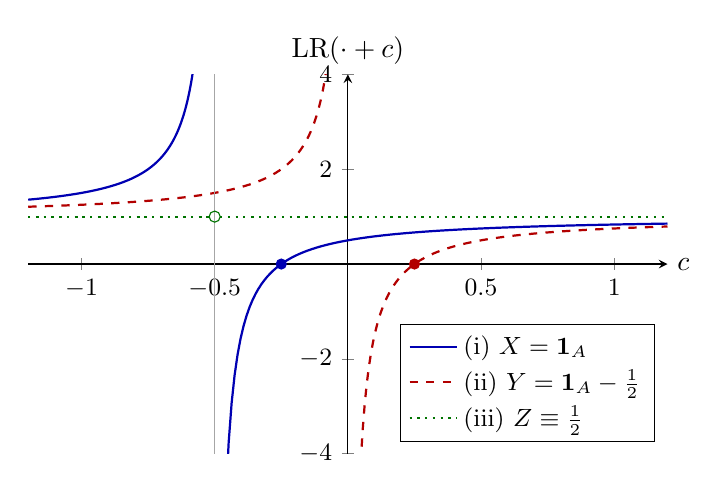
\begin{tikzpicture}
\begin{axis}[width=0.8\textwidth,height=6.4cm,xmin=-1.2,xmax=1.2,ymin=-4,ymax=4,
  axis lines=middle,xtick={-1,-0.5,0,0.5,1},xlabel={$c$},ylabel={$\LR(\cdot+c)$},
  xlabel style={at={(axis cs:1.2,0)},anchor=west},ylabel style={at={(axis cs:0,4)},anchor=south},
  samples=150,unbounded coords=jump,tick label style={font=\small},
  legend style={font=\small,at={(0.98,0.03)},anchor=south east,cells={anchor=west}}]
\addplot[thick,blue!70!black,domain=-1.2:-0.53] {(0.25+x)/(0.5+x)};
\addlegendentry{(i) $X=\1_A$}
\addplot[thick,red!70!black,dashed,domain=-1.2:-0.04] {(x-0.25)/x};
\addlegendentry{(ii) $Y=\1_A-\frac12$}
\addplot[thick,green!45!black,dotted,domain=-1.2:-0.52] {1};
\addlegendentry{(iii) $Z\equiv\frac12$}
\addplot[thick,blue!70!black,domain=-0.47:1.2,forget plot] {(0.25+x)/(0.5+x)};
\addplot[thick,red!70!black,dashed,domain=0.04:1.2,forget plot] {(x-0.25)/x};
\addplot[thick,green!45!black,dotted,domain=-0.48:1.2,forget plot] {1};
\draw[gray!70] (axis cs:-0.5,-4) -- (axis cs:-0.5,4);
\addplot[only marks,mark=*,mark size=1.8pt,blue!70!black,forget plot] coordinates {(-0.25,0)};
\addplot[only marks,mark=*,mark size=1.8pt,red!70!black,forget plot] coordinates {(0.25,0)};
\addplot[only marks,mark=o,mark size=2pt,green!45!black,forget plot] coordinates {(-0.5,1)};
\end{axis}
\end{tikzpicture}
\caption{Cash lines of the three books of Example~\ref{ex:three}. Book (i) explodes at $c=-\frac12$ (its price
point) and vanishes at $c=-\frac14$; book (ii) explodes at $c=0$ with residue $-\frac14$; book (iii) equals $1$
except at its price point $c=-\frac12$, where the singularity is removable (open circle).}\label{fig:three}
\end{figure}

\begin{remark}[Labels at the price point]\label{rem:labels}
To have $\LR=\bracket{\rho}{\Pi}$ also at price points, one may adopt the convention
\begin{center}
\ax{S}\quad at the price point, $\LR=\star$ if the residue in (c) is zero and $\LR=\infty$ otherwise.
\end{center}
Convention \ax{S} is not used in the proofs. If, instead, the loss ratio is real valued with $0/0:=1$, the price
point of a break-even book cannot be observed and the implied premium is not defined there.
\end{remark}

\begin{remark}[A formulation by cash lines]\label{rem:oldCP}
One may alternatively postulate (CP): every cash line is a unit-slope Möbius map,
$\LR(X+c)=\bracket{\rho(X)+c}{\Pi(X)+c}$. Proposition~\ref{prop:readings}(a) shows that (CP) follows from \axP,
\axN{} and \axCM, the labels agreeing under \ax{S}. Conversely, (CP) implies \axP{} and \ax{S}, and (CP) together
with \axCM{} implies \axN: if $\pi_0:=\Pi(0)\ne0$, \axCM{} applied to the constants $a=b=-\pi_0/2$ forces
$\LR(-\pi_0)\in\R$, although $-\pi_0$ is the price point of $0$; hence $\pi_0=0$, and \axCM{} with $X=Y=a\ne0$ gives
$(\rho(0)+2a)/(2a)=(\rho(0)+a)/a$, i.e.\ $\rho(0)=0$ and $\LR(c)=1$. Thus \axP+\axN+\axCM+\ax{S} is equivalent to
(CP)+\axCM.
\end{remark}

\subsection{Axiom \axLI: law invariance}\label{sec:li}

\begin{axiom}[\axLI]\label{ax:LI}
If $X\eqd Y$, then either $\LR(X)=\LR(Y)$ or both values are non-finite.
\end{axiom}

This is the standard assumption of premium and risk-measure theory \citep{wyp1997,kusuoka2001}. Because the
implied premium and risk measure are computed from cash lines, \axLI{} passes to them (Lemma~\ref{lem:LI}).
Ratios that weight scenarios non-uniformly, such as $\E_Q/\E$ with $Q\neq P$, violate \axLI; they are covered by
Theorem~\ref{thm:A0}.

\subsection{Axioms \axRC{} and \axRM: regularity of the implied pair}\label{sec:reg}

Under \axP, write $\rho_D:=\Pi\cdot\LR$ on $D$. The regularity axioms are stated for $\Pi$ and $\rho_D$, so that
they make sense independently of the other axioms.

\begin{axiom}[\axRC]\label{ax:RC}
$\Pi$ is uniformly continuous on $(L^\infty,\|\cdot\|_\infty)$ and $\rho_D$ is uniformly continuous on $D$.
\end{axiom}

\begin{axiom}[\axRM]\label{ax:RM}
If $X\le Y$ almost surely, then $\Pi(X)\le\Pi(Y)$, and $\rho_D(X)\le\rho_D(Y)$ if $X,Y\in D$.
\end{axiom}

Under \axN{} and \axCM{} these axioms are equivalent to the corresponding properties of the implied risk
measure on $L^\infty$, and \axRM{} implies \axRC{} (Lemma~\ref{lem:cashlip}). We include the signed tier
(\axRC) because the canonical family $\rho_\beta$ is a difference of monotone functionals and is in general not
monotone (Corollary~\ref{cor:assoc} and Example~\ref{ex:family}). Monotonicity is imposed on the implied pair and
not on the ratio, for the following reason.

\begin{proposition}[No monotone loss ratio]\label{prop:F2}
Let $h,g\in\Hset_1$ with $g>0$ on $(0,1]$, and let $\LR=I_h/I_g$ on $\Xp:=L^\infty_+\setminus\{0\}$.
If $\LR$ is monotone on $\Xp$ (non-decreasing or non-increasing for the almost sure order),
then $h=g$ and $\LR\equiv1$.
\end{proposition}

\begin{proof}
Let $P(A)=p>0$. For $c\ge0$, $\LR(\1_A+c)=\frac{h(p)+c}{g(p)+c}$ is monotone in $c$ with derivative at
$0$ of the sign of $g(p)-h(p)$. Next let $P(E)=q>0$ and $t\ge0$. Then $X_t=1+t\1_E\in\Xp$ is
increasing in $t$, and $I_k(X_t)=1+t\,k(q)$ for $k\in\{h,g\}$, so
$\LR(X_t)=\frac{1+t\,h(q)}{1+t\,g(q)}$ has derivative at $t=0$ of the sign of $h(q)-g(q)$. If $\LR$
is non-decreasing both signs are non-negative, hence $h=g$ on $(0,1]$; if $\LR$ is non-increasing both are
non-positive, and again $h=g$. \qedhere
\end{proof}

\begin{example}\label{ex:F2}
Let $h=\mathrm{id}$, $g=\sqrt{\cdot}$ and $p=q=\tfrac14$ in the proof. Both families of books in
Figure~\ref{fig:F2} increase in the almost sure order, but the loss ratio increases along the first and
decreases along the second: adding a sure loss to an over-priced book moves the ratio towards $1$ from below,
whereas adding risk to a sure loss moves it away from $1$.
\end{example}

\begin{figure}[ht]
\centering
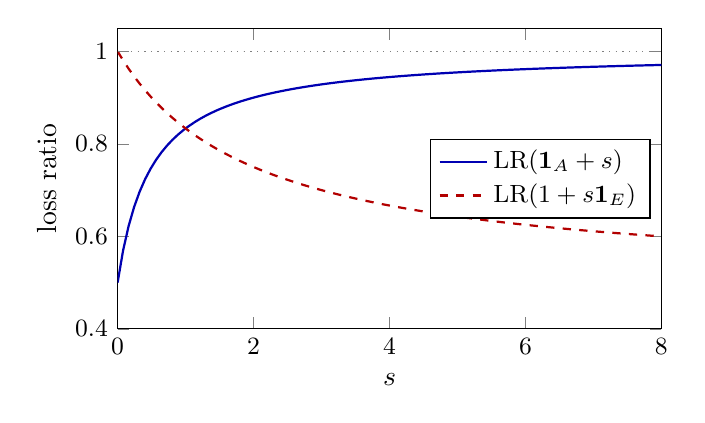
\begin{tikzpicture}
\begin{axis}[width=0.7\textwidth,height=5.4cm,xmin=0,xmax=8,ymin=0.4,ymax=1.05,
  xlabel={$s$},ylabel={loss ratio},tick label style={font=\small},samples=100,domain=0:8,
  legend style={font=\small,at={(0.98,0.5)},anchor=east,cells={anchor=west}}]
\addplot[thick,blue!70!black] {(0.25+x)/(0.5+x)};
\addlegendentry{$\LR(\1_A+s)$}
\addplot[thick,red!70!black,dashed] {(1+0.25*x)/(1+0.5*x)};
\addlegendentry{$\LR(1+s\1_E)$}
\addplot[gray,dotted,domain=0:8] {1};
\end{axis}
\end{tikzpicture}
\caption{Example~\ref{ex:F2}: $h=\mathrm{id}$, $g=\sqrt{\cdot}$, $P(A)=P(E)=\frac14$. Both families of books
increase with $s$; the loss ratio increases along one and decreases along the other.}\label{fig:F2}
\end{figure}

Consequently, the theorems on acceptability indices \citep{chernymadan2009}, which require monotonicity of the
index, do not apply to loss ratios.

\subsection{Summary}

\begin{table}[ht]
\centering\small
\begin{tabularx}{\textwidth}{@{}l>{\raggedright\arraybackslash}p{4.2cm}>{\raggedright\arraybackslash}X@{}}
\toprule
\textbf{Axiom} & \textbf{Statement} & \textbf{Interpretation and counterpart}\\
\midrule
\axP & one price point on each cash line & defines the premium; the level $\beta=\infty$ of the associated family\\
\axN & $\LR(c)=1$ for $c\ne0$ & no unjustified loading \citep{gerber1974}\\
\axCM & comonotone pooling at relative cost & comonotonic additivity \citep{yaari1987,wyp1997}\\
\axLI & law invariance & standard \citep{wyp1997,kusuoka2001}\\
\axRC/\axRM & regularity of the implied pair & continuity / monotonicity of premia\\
\bottomrule
\end{tabularx}
\caption{The axioms.}\label{tab:axioms}
\end{table}

\section{Main results}\label{sec:results}

Throughout this section $\LR:L^\infty\to\widehat{\R}_\star$, and $\Pi$ and $\rho$ denote the implied
premium and the implied risk measure (Definitions~\ref{def:impliedprem} and~\ref{def:impliedrisk},
Proposition~\ref{prop:readings}).

\subsection{The two characterization theorems}

\begin{theorem}[Signed tier]\label{thm:A}
The following are equivalent.
\begin{enumerate}[label=(\roman*),nosep]
\item $\LR$ satisfies \axP, \axN, \axCM, \axLI{} and \axRC.
\item There is a pair $(h,g)\in\Hset_1^2$ such that $\LR(X)=I_h(X)/I_g(X)$ whenever $I_g(X)\neq0$, and
  $\LR(X)\notin\R$ whenever $I_g(X)=0$.
\end{enumerate}
In that case the implied premium is $\Pi=I_g$ and the implied risk measure is $\rho=I_h$. If, in addition,
the labelling convention \ax{S} holds, then $\LR=\bracket{I_h}{I_g}$ on all of $L^\infty$.
\end{theorem}

\begin{theorem}[Distortion tier]\label{thm:B}
The following are equivalent.
\begin{enumerate}[label=(\roman*),nosep]
\item $\LR$ satisfies \axP, \axN, \axCM, \axLI{} and \axRM.
\item Statement (ii) of Theorem~\ref{thm:A} holds with $h,g$ distortion functions (non-decreasing elements
  of $\Hset_1$).
\end{enumerate}
\end{theorem}

The proofs are given in Section~\ref{sec:proofs}; Section~\ref{sec:necessity} shows that none of the axioms
can be dropped.

\subsection{Uniqueness and derived properties}

\begin{proposition}\label{prop:unique}
In Theorems~\ref{thm:A} and~\ref{thm:B}, $(h,g)$ is unique. For an event $A$ with $P(A)=p$,
\begin{align*}
 g(p)&=-c^*,\qquad c^*=\text{the price point of }\1_A;\\
 h(p)&=\big(g(p)+c\big)\,\LR(\1_A+c)-c\qquad\text{for any }c\neq-g(p).
\end{align*}
Moreover $D=\{I_g\ne0\}$ and the break-even set is $N:=\{\rho=\Pi\}=\{I_{h-g}=0\}$. Within
Theorem~\ref{thm:A}, $\rho$ (respectively $\Pi$) is monotone if and only if $h$ (respectively $g$) is
non-decreasing.
\end{proposition}

\begin{proposition}\label{prop:derived}
Under the axioms of Theorem~\ref{thm:A}:
\begin{enumerate}[label=(\roman*),nosep]
\item every cash line is a unit-slope Möbius map, $\LR(X+c)=(\rho(X)+c)/(\Pi(X)+c)$ for $c\ne-\Pi(X)$;
\item $\rho$ and $\Pi$ are cash additive, $\rho(c)=\Pi(c)=c$, and they are Lipschitz with constants
  $\TV(h)$ and $\TV(g)$;
\item $\rho$ and $\Pi$ are comonotonic additive and positively homogeneous, hence $\LR$ is scale invariant:
  $\LR(\lambda X)=\LR(X)$ for $\lambda>0$ and $X\in D$, and for all $X$ under \ax{S}.
\end{enumerate}
\end{proposition}

Properties that are often postulated for the numerator and the denominator of a loss ratio are thus derived;
the association itself is derived in
Corollary~\ref{cor:assoc}.

\subsection{Examples}

\begin{example}[Expected loss over a proportional hazard premium]\label{ex:PH}
Let $h=\mathrm{id}$ and $g_r(p)=p^r$ with $r\in(0,1)$, so that $\rho=\E$ and $\Pi$ is the proportional hazard
premium. For $P(A)=p$, $\LR(\1_A)=p^{1-r}$, and Proposition~\ref{prop:unique} recovers the premium distortion
from the loss ratios of Bernoulli books, $g_r(p)=p/\LR(\1_A)$. For a loss $U$ uniform on $[0,1]$,
$\E U=\tfrac12$ and $\Pi(U)=\int_0^1(1-x)^r\,dx=1/(1+r)$, so $\LR(U)=(1+r)/2$. Since $g_r$ is concave and $h$ is
linear, $\LR\le1$ on $\Xp$ (Corollary~\ref{cor:shape}). The left panel of Figure~\ref{fig:examples} shows
$p\mapsto\LR(\1_A)$ for three values of $r$.
\end{example}

\begin{example}[Expected shortfall over expected loss]\label{ex:ES}
Let $h_\alpha(p)=\min\{p/(1-\alpha),1\}$, $\alpha\in(0,1)$, and $g=\mathrm{id}$, so that $\rho=\mathrm{ES}_\alpha$ and
$\Pi=\E$. Then $\LR(\1_A)=\min\{1/(1-\alpha),1/p\}$ and $\LR(U)=1+\alpha$ for $U$ uniform on $[0,1]$. Here $h_\alpha$ is
concave and $g$ is convex, so $\LR\ge1$ and $\LR$ is quasi-convex on $\{\Pi>0\}$
(Corollary~\ref{cor:shape}(d)); see the right panel of Figure~\ref{fig:examples}.
\end{example}

\begin{figure}[ht]
\centering
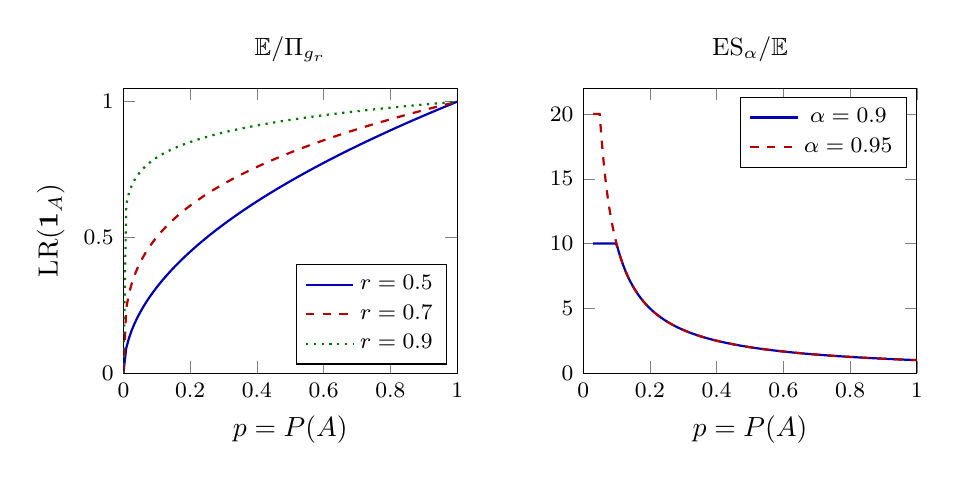
\begin{tikzpicture}
\begin{axis}[name=left,width=0.48\textwidth,height=5.2cm,xmin=0,xmax=1,ymin=0,ymax=1.05,
  xlabel={$p=P(A)$},ylabel={$\LR(\1_A)$},tick label style={font=\footnotesize},samples=120,domain=0:1,
  title={\small $\E/\Pi_{g_r}$},legend style={font=\footnotesize,at={(0.97,0.03)},anchor=south east}]
\addplot[thick,blue!70!black] {x^0.5}; \addlegendentry{$r=0.5$}
\addplot[thick,red!70!black,dashed] {x^0.3}; \addlegendentry{$r=0.7$}
\addplot[thick,green!45!black,dotted] {x^0.1}; \addlegendentry{$r=0.9$}
\end{axis}
\begin{axis}[at={(left.south east)},xshift=1.6cm,width=0.48\textwidth,height=5.2cm,xmin=0,xmax=1,ymin=0,ymax=22,
  xlabel={$p=P(A)$},tick label style={font=\footnotesize},samples=200,domain=0.03:1,
  title={\small $\mathrm{ES}_\alpha/\E$},legend style={font=\footnotesize,at={(0.97,0.97)},anchor=north east}]
\addplot[thick,blue!70!black] {min(1/(1-0.9),1/x)}; \addlegendentry{$\alpha=0.9$}
\addplot[thick,red!70!black,dashed] {min(1/(1-0.95),1/x)}; \addlegendentry{$\alpha=0.95$}
\end{axis}
\end{tikzpicture}
\caption{Loss ratios of Bernoulli books $\1_A$ as functions of $p=P(A)$. Left: expected loss over the
proportional hazard premium (Example~\ref{ex:PH}); the curves identify $g_r(p)=p/\LR(\1_A)$. Right: expected
shortfall over expected loss (Example~\ref{ex:ES}).}\label{fig:examples}
\end{figure}

\subsection{Dropping law invariance}

We state the version without \axLI, which covers scenario-dependent loss ratios. A \emph{game} is a map $\nu:\mathcal F\to\R$ with $\nu(\emptyset)=0$. It is
\emph{null-invariant} if $P(A\triangle B)=0$ implies $\nu(A)=\nu(B)$; its \emph{chain variation} is
$\|\nu\|_{bv}=\sup\sum_j|\nu(A_j)-\nu(A_{j-1})|$ over chains
$\emptyset=A_0\subset\dots\subset A_n=\Omega$. Let $\mathcal V_1$ be the null-invariant games with
$\|\nu\|_{bv}<\infty$ and $\nu(\Omega)=1$, and for $\nu\in\mathcal V_1$ let
$C_\nu(X)=\int_0^\infty\nu(X>x)\,dx+\int_{-\infty}^0[\nu(X>x)-1]\,dx$. A \emph{capacity} is a monotone game.

\begin{theorem}[Without law invariance]\label{thm:A0}
$\LR$ satisfies \axP, \axN, \axCM{} and \axRC{} if and only if $\LR=C_{\nu_1}/C_{\nu_2}$ where
$C_{\nu_2}\ne0$ and $\LR\notin\R$ where $C_{\nu_2}=0$, for $\nu_1,\nu_2\in\mathcal V_1$; with \axRM{} in place
of \axRC{}, if and only if the same holds with capacities $\nu_1,\nu_2$. The pair is unique:
$\nu_1(A)=\rho(\1_A)$ and $\nu_2(A)=\Pi(\1_A)$. The loss ratio is in addition law invariant if and only if
$\nu_i=k_i\circ P$ with $k_i\in\Hset_1$, which recovers Theorems~\ref{thm:A} and~\ref{thm:B}.
\end{theorem}

The set-function representation in Theorem~\ref{thm:A0} is that of \citet{msm1994} and
\citet{cmmm2012,cmmm2015}; the proof is in Appendix~\ref{app:A0}.

\section{On the role of the axioms}\label{sec:triviality}

\subsection{Structure of the result}

The proof of Theorem~\ref{thm:A} has three steps.

\begin{enumerate}[label=(\Alph*),leftmargin=*,itemsep=2pt]
\item \emph{Implied pair.} Axiom \axP{} defines $\Pi$; \axN{} and \axCM{}, applied with sure losses, define $\rho$ and
  give the Möbius form of the cash lines (Lemmas~\ref{lem:premium} and~\ref{lem:implied}).
\item \emph{Transfer.} Given \axP{} and \axN, \axCM{} holds if and only if $\rho$ and $\Pi$ are comonotonic
  additive (Lemma~\ref{lem:comon}), and \axLI{} passes from $\LR$ to $\rho$ and $\Pi$ (Lemma~\ref{lem:LI}).
\item \emph{Representation.} A law-invariant, comonotonic additive, uniformly continuous functional on an
  atomless $L^\infty$ is a signed Choquet integral \citep[Thm.~1]{www2020}; under monotonicity it is a
  distortion premium \citep{schmeidler1986,wyp1997}.
\end{enumerate}

Step (C) is classical; we reprove it in Section~\ref{sec:proofs} to keep the constants explicit and to show that
no continuity is needed in the monotone case. Steps (A) and (B) are specific to loss ratios. Together, axioms
\axP, \axN{} and \axCM{} state that $\LR$ is the ratio of a pair of comonotonic additive functionals that coincide
with the identity on constants, and that this pair can be read off $\LR$.

\subsection{Assumed and derived properties}

Table~\ref{tab:derived} lists the properties of the representation and their source. Axiom \axP{} is ordinal and
serves as a definition, \axN{} is a normalization, and \axLI, \axRC, \axRM{} select the class of representing
functions. The cardinal content of the axioms lies in \axCM: given \axP{} and \axN, it is equivalent to
comonotonic additivity of the implied premium and risk measure, which is the axiom that produces Choquet
representations in \citet{yaari1987}, \citet{schmeidler1986} and \citet{wyp1997}. The Choquet form of the numerator
and the denominator is therefore a consequence of comonotonic additivity, as in the single-functional case.

\begin{table}[ht]
\centering\small
\begin{tabularx}{\textwidth}{@{}>{\raggedright\arraybackslash}p{4.8cm}>{\raggedright\arraybackslash}X>{\raggedright\arraybackslash}p{2.0cm}@{}}
\toprule
\textbf{Property} & \textbf{Source} & \textbf{Status}\\
\midrule
$\Pi$ exists and is cash additive & \axP{} & definition\\
$\Pi(c)=c$, $\rho(c)=c$ & \axN{} and \axP & derived\\
$\rho$ defined on $L^\infty$; Möbius cash lines & \axCM{} with sure losses (Prop.~\ref{prop:readings}) & derived\\
$\rho,\Pi$ comonotonic additive & \axCM{} (Lemma~\ref{lem:comon}) & equivalent\\
$\rho,\Pi$ law invariant & \axLI{} (Lemma~\ref{lem:LI}) & assumed\\
$\rho,\Pi$ continuous or monotone & \axRC, \axRM{} & assumed\\
$h,g$ of bounded variation & Lemma~\ref{lem:bv} & derived\\
$\rho=I_h$, $\Pi=I_g$ & Lemmas~\ref{lem:layer} and~\ref{lem:rep} & derived\\
positive homogeneity, scale invariance & Lemma~\ref{lem:cashlip} & derived\\
association & Corollary~\ref{cor:assoc} & derived\\
uniqueness of $(h,g)$ & Proposition~\ref{prop:unique} & derived\\
\bottomrule
\end{tabularx}
\caption{Assumed and derived properties in Theorem~\ref{thm:A}.}\label{tab:derived}
\end{table}

\subsection{Relation to the single-functional theory}

The characterizations in the literature concern premiums and risk measures; they cannot be applied to $\LR$
directly, since a loss ratio is not additive and \axCM{} is a weighted-mean identity. What is specific to the
loss ratio is the construction of the implied pair, the derivation of additivity on all comonotone pairs, in
particular on the break-even set where the weights of \axCM{} are not identified (Remark~\ref{rem:primitive}),
uniqueness of $(h,g)$ also when $\LR\equiv1$, the impossibility of a monotone loss ratio
(Proposition~\ref{prop:F2}), the structure of the associated family (Corollary~\ref{cor:assoc}), and the version
for nonnegative losses (Section~\ref{sec:actuarial}), in which the price point is not observed and must be
extrapolated.

\subsection{Loss ratios excluded and included}

Ratios with a proportional loading, $\E/((1+\theta)\E)$, violate \axN; scenario-weighted ratios $\E_Q/\E$ violate
\axLI; the ratio $\max(I_{\sqrt t},I_{\min(1,1.5t)})/\E$ violates \axCM, its numerator being cash additive but not
comonotonic additive; and ordinal transforms such as $(\rho/\Pi)^3$ satisfy \axP{} and \axN{} but violate \axCM.
The class characterized contains, among others, the expected loss over any distortion premium
(Example~\ref{ex:PH}), ratios of expected shortfalls (Example~\ref{ex:ES}), value-at-risk over expected shortfall,
and ratios that take values on both sides of $1$.

\section{Proofs of the main results}\label{sec:proofs}

Figure~\ref{fig:flow} shows the structure of the proof. Lemmas~\ref{lem:premium}--\ref{lem:LI} are
specific to loss ratios; Lemmas~\ref{lem:cashlip}--\ref{lem:rep} reprove the representation of comonotonic
additive functionals in the form needed here.

\begin{figure}[ht]
\centering\small
\fbox{\begin{minipage}{0.92\textwidth}\centering
\textbf{Lemma~\ref{lem:premium}} (implied premium): $\Pi$ from the price point; cash additive; $\Pi(c)=c$\ \ (\axP, \axN)\\[2pt]
$\Downarrow$\\[2pt]
\textbf{Lemma~\ref{lem:implied}} (implied risk measure): $\rho=\Pi\cdot\LR$ extends; Möbius cash lines\ \ (\axCM{} with sure losses)\\[2pt]
$\Downarrow$\\[2pt]
\textbf{Lemma~\ref{lem:comon}}: $\rho,\Pi$ comonotonic additive, also on the break-even set\ \ (\axCM)\\[2pt]
$\Downarrow$\\[2pt]
\textbf{Lemma~\ref{lem:LI}}: $\rho,\Pi$ law invariant\ \ (\axLI)\\[2pt]
$\Downarrow$\\[2pt]
\textbf{Lemma~\ref{lem:cashlip}}: homogeneity, Lipschitz\ \ (\axRC{} or \axRM)\\[2pt]
$\Downarrow$\\[2pt]
\textbf{Lemma~\ref{lem:layer}}: layer formula; $h(p)=\rho(\1_A)$, $g(p)=\Pi(\1_A)$\ \ $\Rightarrow$\ \
\textbf{Lemma~\ref{lem:bv}}: bounded variation\ \ $\Rightarrow$\ \ \textbf{Lemma~\ref{lem:rep}}: $\rho=I_h$, $\Pi=I_g$
\end{minipage}}
\caption{Logical structure of the proof of Theorems~\ref{thm:A} and~\ref{thm:B}.}\label{fig:flow}
\end{figure}

\begin{lemma}[Implied premium]\label{lem:premium}
Assume \axP. Then $\Pi(X+c)=\Pi(X)+c$ for all $X$ and $c$, and $D=\{\Pi\ne0\}$. If also \axN, then
$\Pi(c)=c$ for every constant $c$.
\end{lemma}

\begin{proof}
The cash line of $X+c$ is $d\mapsto\LR(X+c+d)$, the cash line of $X$ shifted by $c$; its price point is
therefore the price point of $X$ minus $c$, which is \eqref{eq:Picash}. $X\in D$ means that $0$ is not the
price point, i.e.\ $\Pi(X)\ne0$. Under \axN{} the cash line of $0$ takes the value $1$ at every $d\neq0$, so
its price point is $0$, $\Pi(0)=0$, and $\Pi(c)=c$. \qedhere
\end{proof}

\begin{lemma}[Implied risk measure]\label{lem:implied}
Assume \axP, \axN, \axCM. If $X\in D$ and $X+c\in D$, then $\rho(X+c)=\rho(X)+c$. Consequently
$\rho(X):=\rho(X+c)-c$, for any $c\ne-\Pi(X)$, defines a cash-additive functional on $L^\infty$ that agrees
with $\Pi\cdot\LR$ on $D$, satisfies $\rho(c)=c$, and
\begin{equation}\label{eq:mobius}
 \LR(X+c)=\frac{\rho(X)+c}{\Pi(X)+c}\qquad\text{for all }c\ne-\Pi(X).
\end{equation}
\end{lemma}

\begin{proof}
Let $X,X+c\in D$ with $c\ne0$. The constant $c$ lies in $D$ (by \axN), is comonotone with $X$, and
$\Pi(X)+\Pi(c)=\Pi(X+c)\ne0$ by Lemma~\ref{lem:premium}. So \axCM{} applies to the pair $(X,c)$ and gives
$\LR(X+c)=(\Pi(X)\LR(X)+c)/(\Pi(X)+c)$, i.e.\ $\rho(X+c)=\Pi(X+c)\LR(X+c)=\rho(X)+c$.

For arbitrary $X$, $X+c\in D$ exactly when $c\ne-\Pi(X)$. If $c,c'$ are two such values, then
$X+c'=(X+c)+(c'-c)$ with both $X+c$ and $X+c'$ in $D$, so $\rho(X+c')=\rho(X+c)+(c'-c)$; hence
$\rho(X+c)-c$ does not depend on $c$, and for $X\in D$ (take $c=0$) it equals $\Pi(X)\LR(X)$. Cash additivity
of the extension is immediate. For $c\neq-\Pi(X)$,
$\LR(X+c)=\rho(X+c)/\Pi(X+c)=(\rho(X)+c)/(\Pi(X)+c)$. Finally $\rho(c)=\Pi(c)\LR(c)=c$ for $c\ne0$, and
$\rho(0)=\rho(1)-1=0$. \qedhere
\end{proof}

\begin{proof}[Proof of Proposition~\ref{prop:readings}]
(a) is \eqref{eq:mobius}, and (b) restates it. For (c), $(c+\Pi(X))\LR(X+c)=\rho(X)+c\to\rho(X)-\Pi(X)$ as
$c\to-\Pi(X)$. For (d), the right-hand side of \eqref{eq:mobius} vanishes only at $c=-\rho(X)$, which differs
from the price point when $\rho(X)\ne\Pi(X)$; when $\rho(X)=\Pi(X)$ it equals $1$ for every $c\ne-\Pi(X)$.
Uniqueness of the extension is clear, since any cash-additive extension must satisfy (b). \qedhere
\end{proof}

\begin{lemma}[Comonotonic additivity]\label{lem:comon}
Assume \axP{} and \axN.
\begin{enumerate}[label=(\alph*),nosep]
\item If \axCM{} holds, then $\rho$ and $\Pi$ are comonotonic additive.
\item Conversely, if $\Pi$ is comonotonic additive and there is a comonotonic additive $\tilde\rho$ with
  $\tilde\rho=\Pi\cdot\LR$ on $D$, then \axCM{} holds and the implied risk measure equals $\tilde\rho$.
\end{enumerate}
\end{lemma}

\begin{proof}
(a) Let $X,Y$ be comonotone, $Z=X+Y$, $r=\rho(X)+\rho(Y)$ and $q=\Pi(X)+\Pi(Y)$. Fix $s\neq-q$ and choose
$u\notin\{-\Pi(X),\,s+\Pi(Y)\}$.
\begin{enumerate}[label=(\arabic*),nosep]
\item $X+u$ and $Y+s-u$ are comonotone, and by Lemma~\ref{lem:premium} their premiums $\Pi(X)+u$ and
  $\Pi(Y)+s-u$ are non-zero. So both lie in $D$, and their premiums sum to $q+s\neq0$.
\item Apply \axCM{} to this pair and use $\rho=\Pi\cdot\LR$ on $D$ with Lemma~\ref{lem:implied}:
  \[
  \LR(Z+s)=\frac{(\rho(X)+u)+(\rho(Y)+s-u)}{q+s}=\frac{r+s}{q+s}\in\R .
  \]
\item Thus the cash line of $Z$ is finite at every $s\neq-q$. By \axP{} it has exactly one non-finite
  point, so that point is $-q$, and $\Pi(Z)=q$.
\item For $s\ne-q$, Lemma~\ref{lem:implied} gives $\rho(Z)+s=\rho(Z+s)=\Pi(Z+s)\LR(Z+s)=r+s$, so $\rho(Z)=r$.
\end{enumerate}
The argument never asks whether $X$, $Y$ or $Z$ break even: \axP{} locates the price point even when the
cash line equals $1$ everywhere else.

(b) Let $X,Y\in D$ be comonotone with $q=\Pi(X)+\Pi(Y)\ne0$. Then $\Pi(X+Y)=q\ne0$, so $X+Y\in D$, and
$\LR(X+Y)=\tilde\rho(X+Y)/q=(\tilde\rho(X)+\tilde\rho(Y))/q=(\Pi(X)\LR(X)+\Pi(Y)\LR(Y))/q$. Both $\tilde\rho$ and
the implied risk measure are cash additive (the former by additivity with constants and $\tilde\rho(c)=\Pi(c)\LR(c)=c$)
and agree on $D$, hence everywhere. \qedhere
\end{proof}

\begin{lemma}[Law invariance of the implied pair]\label{lem:LI}
Assume \axP, \axN, \axCM{} and \axLI. Then $\rho$ and $\Pi$ are law invariant.
\end{lemma}

\begin{proof}
If $X\eqd Y$ then $X+c\eqd Y+c$ for every $c$, so by \axLI{} the cash lines of $X$ and $Y$ have the same finite
values and the same non-finite locations. Hence they have the same price point, $\Pi(X)=\Pi(Y)$, and by Proposition~\ref{prop:readings}(b) $\rho(X)=\rho(Y)$. \qedhere
\end{proof}

\begin{lemma}[Homogeneity and Lipschitz continuity]\label{lem:cashlip}
Assume \axP, \axN, \axCM, and let $F\in\{\rho,\Pi\}$. If \axRC{} or \axRM{} holds, $F$ is positively homogeneous
and Lipschitz; under \axRM{} it is $1$-Lipschitz.
\end{lemma}

\begin{proof}
First, the axioms transfer from $\rho_D$ to $\rho$. Given $X,Y$, choose $c$ with $|c|$ arbitrarily small and
$X+c,Y+c\in D$ (only two values are excluded). Then $\rho(X)-\rho(Y)=\rho_D(X+c)-\rho_D(Y+c)$ with
$\|(X+c)-(Y+c)\|=\|X-Y\|$, and $X\le Y$ implies $X+c\le Y+c$; so $\rho$ is uniformly continuous with the modulus
of $\rho_D$ under \axRC, and monotone under \axRM.
Since $X$ is comonotone with itself, $F(nX)=nF(X)$ by Lemma~\ref{lem:comon}, so $F(qX)=qF(X)$ for rational $q>0$.
\emph{Under \axRM:} $X\le Y+\|X-Y\|$ gives $F(X)\le F(Y)+\|X-Y\|$ by monotonicity and cash additivity, so $F$ is
$1$-Lipschitz, and homogeneity extends to real $\lambda>0$. \emph{Under \axRC:} continuity gives
$F(\lambda X)=\lambda F(X)$ for real $\lambda>0$. Choose $\delta>0$ with $|F(X')-F(Y')|\le1$ whenever
$\|X'-Y'\|\le\delta$, and apply it to $tX,tY$ with $t=\delta/\|X-Y\|$; this gives
$|F(X)-F(Y)|\le\|X-Y\|/\delta$. \qedhere
\end{proof}

\begin{lemma}[Layer formula]\label{lem:layer}
Assume \axP, \axN, \axCM, \axLI{} and \axRC{} (or \axRM). Define, for $P(A)=p$, $h(p):=\rho(\1_A)$ and
$g(p):=\Pi(\1_A)$. These are well defined by Lemma~\ref{lem:LI}, defined for every $p\in[0,1]$ because the
space is atomless, and $h(0)=g(0)=0$, $h(1)=g(1)=1$. For every chain $C_1\supset\dots\supset C_m$, $x_0\in\R$
and $a_i\ge0$,
\begin{equation}\label{eq:layer}
 \rho\Big(x_0+\sum_i a_i\1_{C_i}\Big)=x_0+\sum_i a_i\,h(P(C_i)),
\end{equation}
and likewise for $\Pi$ with $g$.
\end{lemma}

\begin{proof}
The partial sum $S_{j-1}=\sum_{i<j}a_i\1_{C_i}$ attains its maximum on $C_j$, so it is comonotone with
$\1_{C_j}$. Apply Lemma~\ref{lem:comon} and cash additivity successively, with
$\rho(a\1_C)=a\rho(\1_C)=a\,h(P(C))$ by Lemma~\ref{lem:cashlip}. The values at $0$ and $1$ come from
$\rho(0)=\Pi(0)=0$ and $\rho(1)=\Pi(1)=1$. \qedhere
\end{proof}

\begin{lemma}[Bounded variation]\label{lem:bv}
Under the assumptions of Lemma~\ref{lem:layer}, $h,g\in\Hset_1$. Under \axRM{} they are non-decreasing.
\end{lemma}

\begin{proof}
\emph{Under \axRM.} For $p\le q$ choose nested $A\subset B$ with $P(A)=p$, $P(B)=q$; then $\1_A\le\1_B$ gives
$h(p)\le h(q)$, and likewise for $g$.

\emph{Under \axRC.} Let $L$ be a Lipschitz constant of $\rho$. Take $0=p_0<\dots<p_n=1$ and a uniform random
variable $U$. Put $I_j=\{1-p_j<U\le1-p_{j-1}\}$ and $\delta_j=h(p_j)-h(p_{j-1})$. For $\sigma\in\{0,1\}^n$ let
$W=\sum_j2(n-j)\1_{I_j}$ and $Y_\sigma=W+\sum_j\sigma_j\1_{I_j}$. The values $2(n-j)+\sigma_j$ are strictly
decreasing in $j$, so $W$ and $Y_\sigma$ have the same upper sets $\{U>1-p_j\}$, of probability $p_j$. By
\eqref{eq:layer} and summation by parts, $\rho\big(\sum_jv_j\1_{I_j}\big)=\sum_jv_j\delta_j$ for every
non-increasing $v\ge0$. Hence $|\sum_j\sigma_j\delta_j|=|\rho(Y_\sigma)-\rho(W)|\le L\|Y_\sigma-W\|\le L$.
Choosing $\sigma_j=\1\{\delta_j>0\}$ and then $\sigma_j=\1\{\delta_j<0\}$ gives $\sum_j|\delta_j|\le2L$. \qedhere
\end{proof}

\begin{lemma}[Representation]\label{lem:rep}
Under the assumptions of Lemma~\ref{lem:layer}, $\rho=I_h$ and $\Pi=I_g$.
\end{lemma}

\begin{proof}
For a simple $X=x_0+\sum_ia_i\1_{C_i}$ with $a_i\ge0$ and $C_i=\{X\ge x_i\}$, a direct computation gives
$I_h(X)=x_0+\sum_ia_ih(P(C_i))=\rho(X)$. Simple positions are uniformly dense in $L^\infty$, and $\rho$ and
$I_h$ are both Lipschitz (Lemma~\ref{lem:cashlip} and $|I_h(X)-I_h(Y)|\le\TV(h)\|X-Y\|$), so $\rho=I_h$.
Likewise $\Pi=I_g$. \qedhere
\end{proof}

\begin{proof}[Proof of Theorems~\ref{thm:A} and~\ref{thm:B}]
\emph{(i)$\Rightarrow$(ii).} Lemmas~\ref{lem:premium}--\ref{lem:rep} give $\Pi=I_g$ and $\rho=I_h$ with
$h,g\in\Hset_1$, non-decreasing under \axRM. On $D=\{\Pi\ne0\}=\{I_g\ne0\}$, $\LR=\rho/\Pi=I_h/I_g$, and off $D$
the loss ratio is not finite. Under \ax{S}, at a book with $I_g(X)=0$ the label is $\star$ exactly when the
residue $\rho(X)=I_h(X)$ vanishes, which is the value of $\bracket{I_h(X)}{0}$.

\emph{(ii)$\Rightarrow$(i).} Let $\LR$ be as in (ii). Since $I_g(X+c)=I_g(X)+c$, the cash line of $X$ is non-finite
exactly at $c=-I_g(X)$, so \axP{} holds and $\Pi=I_g$. \axN{} holds because $I_h(c)=I_g(c)=c$. Next, $I_k$ is
comonotonic additive for $k\in\Hset$: for comonotone $X,Y$, any two upper sets $\{X\ge a\}$, $\{Y\ge b\}$ are almost
surely nested (otherwise comonotonicity fails on a $P\otimes P$-positive set); for simple comonotone $X,Y$ the
union of their upper sets is therefore a chain, giving $X=x_0+\sum a_i\1_{C_i}$, $Y=y_0+\sum b_i\1_{C_i}$ with
$a_i,b_i\ge0$, and additivity follows from the layer computation; for general $X,Y$ approximate by the comonotone
simple pairs $\lfloor nX\rfloor/n$, $\lfloor nY\rfloor/n$ and use the Lipschitz bound. Lemma~\ref{lem:comon}(b) with
$\tilde\rho=I_h$ gives \axCM{} and $\rho=I_h$. \axLI{} holds because $I_k$ depends on $X$ only through
$x\mapsto P(X>x)$, \axRC{} because $I_h,I_g$ are Lipschitz, and \axRM{} when $h,g$ are non-decreasing. \qedhere
\end{proof}

\begin{proof}[Proof of Propositions~\ref{prop:unique} and~\ref{prop:derived}]
$g(p)=\Pi(\1_A)$ is minus the price point of $\1_A$, and $h(p)=\rho(\1_A)$ is given by
Proposition~\ref{prop:readings}(b); both are determined by $\LR$, including when $h=g$. The identities for $D$ and
$N$ follow from $\Pi=I_g$, $\rho=I_h$. Monotonicity of $\rho$ is equivalent to monotonicity of $h$ because $I_h$ is
monotone if and only if $h$ is non-decreasing. Proposition~\ref{prop:derived} collects
Lemmas~\ref{lem:premium}--\ref{lem:comon} and~\ref{lem:cashlip}, the Lipschitz bound for $I_k$, and
$\LR(\lambda X)=\lambda\rho(X)/(\lambda\Pi(X))=\LR(X)$ on $D$ (and $\lambda D=D$). \qedhere
\end{proof}

\section{Nonnegative losses}\label{sec:actuarial}

Insurance losses are nonnegative and premiums are positive. On $\Xp=L^\infty_+\setminus\{0\}$ only upward
shifts $X+c$, $c\ge0$, are available, and the price point $-\Pi(X)<0$ lies outside the domain, so that \axP{}
cannot be used. In this section the loss ratio is a map $\LR_0:\Xp\to\R$, and $N_0:=\{X\in\Xp:\LR_0(X)=1\}$.

\subsection{Axioms}

\begin{definition}[Axioms (A0)--(A5)]\label{def:Axioms}
\begin{description}[leftmargin=0pt,labelindent=0pt,itemsep=3pt,style=unboxed]
\item[(A0)] $N_0$ has empty interior in $(\Xp,\|\cdot\|_\infty)$.
\item[(A1)] For each $X\in\Xp\setminus N_0$ there are reals $a_X,b_X$ with $\LR_0(X+c)=(a_X+c)/(b_X+c)$ for all
  $c\ge0$. By Lemma~\ref{lem:halfline}, $a_X\ne b_X$, the pair is unique and $b_X>0$; put $\rho(X):=a_X$ and
  $\Pi(X):=b_X$ on $\Xp\setminus N_0$.
\item[(A2)] $\LR_0$ is law invariant.
\item[(A3)] $\rho$ and $\Pi$ are non-decreasing on $\Xp\setminus N_0$. Variant (A3$_s$): $\rho$ and $\Pi$ are
  uniformly continuous on $\Xp\setminus N_0$.
\item[(A4)] Let $\bar\rho,\bar\Pi$ be the continuous extensions of $\rho,\Pi$ to $\Xp$ (they exist under (A3) or
  (A3$_s$) by Lemma~\ref{lem:ext}). For comonotone $X,Y\in\Xp$:
  \begin{itemize}[nosep]
  \item[(A4a)] $\bar\Pi(X+Y)=\bar\Pi(X)+\bar\Pi(Y)$;
  \item[(A4b)] $\bar\Pi(X+Y)\LR_0(X+Y)=\bar\Pi(X)\LR_0(X)+\bar\Pi(Y)\LR_0(Y)$.
  \end{itemize}
\item[(A5)] $\LR_0$ is norm-continuous on $\Xp$.
\end{description}
\end{definition}

Axiom (A0) excludes $\LR_0\equiv1$, for which $\rho$ and $\Pi$ are not identified, and ensures that $\rho,\Pi$ are
defined on a dense set. Axiom (A1) is the counterpart of Proposition~\ref{prop:readings}(a) on a half line: since
the price point is not observed, the premium must be extrapolated from $c\ge0$, which requires the functional
form to be assumed rather than derived. Axiom (A4b) is the pooling identity \axCM, and (A4a) states that premiums
add under comonotone pooling; on $\Xp$ the two must be stated separately. Axiom (A5) excludes jumps of $\LR_0$
where the premium distortion vanishes; it excludes, for example, value-at-risk-type premium distortions
$g=\1_{(a,1]}$, and it implies $g>0$ (Step C5 in Appendix~\ref{app:C}).

\begin{lemma}\label{lem:halfline}
If $X\notin N_0$ satisfies (A1) with $(a,b)$, then $a\ne b$, the pair is unique, $b>0$, and for every
$c_0\ge0$ one has $X+c_0\notin N_0$ with $\rho(X+c_0)=\rho(X)+c_0$ and $\Pi(X+c_0)=\Pi(X)+c_0$.
\end{lemma}

\subsection{Results}

\begin{theorem}\label{thm:C}
$\LR_0$ satisfies (A0)--(A5) if and only if $\LR_0=C_h/C_g$ on $\Xp$ for distortion functions $h\ne g$
with $g>0$ on $(0,1]$. In that case $(h,g)$ is unique, also among pairs in $\Hset_1^2$ with
$C_{g'}>0$ on $\Xp$; moreover $\bar\rho=C_h$, $\bar\Pi=C_g$ and $N_0=\Xp\cap\{C_h=C_g\}$.
\end{theorem}

\begin{theorem}\label{thm:Cp}
Axioms (A0)--(A2), (A3$_s$), (A4) and (A5) hold if and only if $\LR_0=C_h/C_g$ with $h,g\in\Hset_1$, $h\ne g$,
and $g>0$ on $(0,1]$.
\end{theorem}

\begin{proposition}\label{prop:bridge}
$\LR_0=C_h/C_g$ with distortion functions $h,g$ and $g>0$ on $(0,1]$ if and only if $\LR_0$ is the restriction to
$\Xp$ of an extended loss ratio satisfying the axioms of Theorem~\ref{thm:B} with $\Pi>0$ on $\Xp$. The representing
pair $(h,g)$ of such an extension is unique if and only if $\LR_0\not\equiv1$. In that case the extension is unique up
to the labels $\infty,\star$ at its non-finite values, and unique under convention \ax{S}.
\end{proposition}

Theorem~\ref{thm:C} is the loss-ratio analogue of the characterization of \citet{wyp1997}. Unlike that result,
the pair $(\rho,\Pi)$ is defined only off $N_0$, and positivity of $g$ is derived from (A5). The proofs are given in
Appendix~\ref{app:C}, and Section~\ref{sec:necessity} shows that none of (A2)--(A5) can be dropped.

\section{Independence of the axioms}\label{sec:necessity}

For each of the axioms \axN, \axCM, \axLI, \axRC{} and \axRM{} we give a loss ratio that satisfies the
remaining axioms and is not of the form in Theorem~\ref{thm:A} or~\ref{thm:B}. Axiom \axP{} defines the implied
premium, through which the other axioms are formulated, and is therefore not treated in the same way; see
Remark~\ref{rem:labels} for what is lost without it. Table~\ref{tab:witnesses} summarizes the examples.

\begin{table}[ht]
\centering\small
\begin{tabularx}{\textwidth}{@{}l>{\raggedright\arraybackslash}p{4.6cm}>{\raggedright\arraybackslash}X@{}}
\toprule
\textbf{Dropped} & \textbf{Witness} & \textbf{Why it is a witness}\\
\midrule
\axN & $\bracket{I_h}{\kappa I_g}$, $\kappa>0$, $\kappa\ne1$
 & All other axioms hold; $\LR(c)=1/\kappa\ne1$.\\
\axCM & $\bracket{\max(I_{\sqrt t},I_{\min(1,1.5t)})}{\E}$
 & Implied risk measure is cash additive but not comonotonic additive.\\
\axLI & $\bracket{\E_Q}{\E}$, $Q\ne P$ with bounded density
 & All other axioms hold; $\E_Q$ is not law invariant.\\
\axRC{} (Thm.~\ref{thm:A}) & $\bracket{I_h}{\E}$ with $h$ continuous, not of bounded variation
 & Uniform continuity fails; $h$ is not of bounded variation.\\
\axRM{} (Thm.~\ref{thm:B}) & $\bracket{I_h}{\E}$, $h(t)=t+\tfrac14\sin2\pi t$
 & $h$ is not monotone, so no distortion pair represents it.\\
\bottomrule
\end{tabularx}
\caption{Witnesses for the axioms of Theorems~\ref{thm:A} and~\ref{thm:B}.}\label{tab:witnesses}
\end{table}

\begin{example}[Independence of \axN: a loading on sure losses]
Fix $\kappa>0$, $\kappa\neq1$, and let $\LR=\bracket{I_h}{\kappa I_g}$ with distortions $h,g$. The cash line of
$X$ is $(I_h(X)+c)/(\kappa(I_g(X)+c))$, non-finite only at $c=-I_g(X)$, so \axP{} holds with $\Pi=I_g$. With these
weights the pooling identity holds because $I_h$ and $I_g$ are comonotonic additive; \axLI{} holds, and so do
\axRM{} and \axRC, since $\Pi=I_g$ and $\rho_D=\Pi\cdot\LR=I_h/\kappa$ are monotone and Lipschitz. But $\LR(c)=1/\kappa\ne1$, whereas every ratio in Theorem~\ref{thm:A} has value $1$ at sure losses. So the
normalization is not harmless: it is what excludes loadings on sure losses. (We conjecture, but have not proved,
that an analogue of Theorem~\ref{thm:A} with a known loading $\kappa$ holds with $\LR=\bracket{I_h}{\kappa I_g}$.)
\end{example}

\begin{example}[Ordinal information is not enough]\label{ex:cube}
Let $h\ne g$ be distortions and $\LR'=\psi\circ\bracket{I_h}{I_g}$ with $\psi(t)=t^3$ and $\psi$ fixing the
non-finite values. Since $\psi$ maps $\R$ to $\R$, $\LR'$ has the same price points as $\bracket{I_h}{I_g}$, so
\axP{} holds with $\Pi=I_g$; \axN{} holds because $1^3=1$; \axLI{} holds, and so does the mediant inequality,
because $\psi$ is increasing. But $\LR'$ is not of the form in Theorem~\ref{thm:A}: at a book $X$ with
$I_h(X)\neq I_g(X)$ (for instance an indicator at a point where $h\ne g$), the cash line
$\big((I_h(X)+c)/(I_g(X)+c)\big)^3$ has a pole of order three, while every cash line in Theorem~\ref{thm:A} has a
simple pole. Hence \axCM{} fails. (This example is an illustration, not a witness in the strict sense: on
$D$, $\Pi\cdot\LR'=I_h^3/I_g^2$ is neither uniformly continuous nor monotone.) Betweenness-type, ordinal information determines the loss ratio only up to an
increasing transformation, as for \citet{chew1983} and \citet{dekel1986}; the cardinal axiom \axCM{} cannot be
avoided.
\end{example}

\begin{example}[Independence of \axCM]
Let $\LR=\bracket{\rho}{\E}$ with $\rho=\max(I_{\sqrt t},I_{\min(1,1.5t)})$. \axP{} holds with $\Pi=\E$, \axN{}
holds, and the implied risk measure is $\rho$, a maximum of cash-additive maps; \axLI, \axRM{} and \axRC{} hold. Take
$E\subset B$ with $P(B)=0.5$, $P(E)=0.1$ and $X=\1_B+\1_E$. Then $\rho(\1_B)=\max(0.707,0.75)=0.75$ and
$\rho(\1_E)=\max(0.316,0.15)=0.316$, with sum $1.066$, while $\rho(X)=\max(0.707+0.316,\ 0.75+0.15)=1.023$. So $\rho$
is not comonotonic additive and \axCM{} fails by Lemma~\ref{lem:comon}(a).
\end{example}

\begin{example}[Independence of \axLI]
Let $Z=dQ/dP$ be bounded, non-constant, $Z\ge0$ and $\E Z=1$, and $\LR=\bracket{\E_Q}{\E}$. \axP{} holds with
$\Pi=\E$, \axN{} holds, \axCM{} holds by Lemma~\ref{lem:comon}(b) because $\E_Q$ and $\E$ are additive, and \axRM,
\axRC{} hold. But $\E_Q(\1_A)=Q(A)$ is not a function of $P(A)$, so the implied risk measure is not of the form
$I_h$. Without \axLI{} the class is exactly that of Theorem~\ref{thm:A0}.
\end{example}

\begin{example}[Independence of \axRC{} in Theorem~\ref{thm:A}]
Let $h(t)=t\big(1+\tfrac12\sin(1/t)\big)/\big(1+\tfrac12\sin1\big)$, continuous with $h(0)=0$, $h(1)=1$, and not of
bounded variation (Figure~\ref{fig:witness}) ($\int|h'|$ diverges at $0$). Let $\LR=\bracket{I_h}{\E}$. \axP, \axN{} and \axLI{} are clear;
$I_h$ is norm continuous (survival functions converge off a countable set, and dominated convergence applies)
and additive on simple comonotone positions by the layer computation, hence comonotonic additive, so \axCM{}
holds. The implied risk measure is $I_h$, and by Lemma~\ref{lem:bv} \axRC{} would force $h$ to be of bounded
variation. So \axRC{} fails and no pair in $\Hset_1^2$ represents $\LR$.
\end{example}

\begin{remark}[Some regularity is indispensable]
\axP, \axN, \axCM{} and \axLI{} alone do not force continuity. Using a Hamel basis one obtains
$\rho=\E+\varphi\circ I_k$ with $k(t)=t(1-t)$ (so that $I_k$ vanishes on constants and is cash invariant) and
$\varphi$ additive but discontinuous. Then $\bracket{\rho}{\E}$ satisfies \axP, \axN, \axCM{} and \axLI{} and is not of
the form in Theorem~\ref{thm:A}. This witness uses the axiom of choice; all the others are constructive.
\end{remark}

\begin{example}[Independence of \axRM{} in Theorem~\ref{thm:B}]
Let $h(t)=t+\tfrac14\sin2\pi t\in\Hset_1$ (Figure~\ref{fig:witness}), so $h(0.4)\approx0.547>h(0.6)\approx0.453$, and
$\LR=\bracket{I_h}{\E}$. All other axioms hold (\axRC{} by the Lipschitz bound), but the implied risk measure
$I_h$ is not monotone, and no distortion pair represents $\LR$ because the pair is unique.
\end{example}

\begin{figure}[ht]
\centering
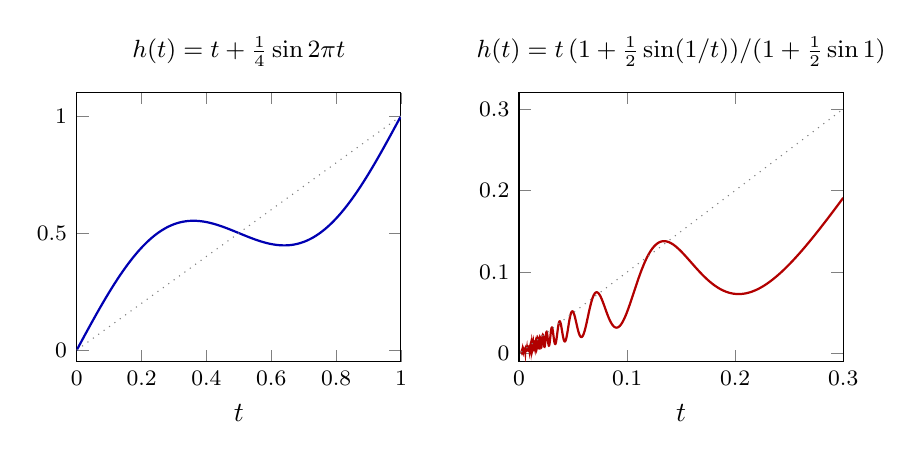
\begin{tikzpicture}
\begin{axis}[name=l,width=0.47\textwidth,height=5cm,xmin=0,xmax=1,ymin=-0.05,ymax=1.1,xlabel={$t$},
  title={\small $h(t)=t+\frac14\sin2\pi t$},tick label style={font=\footnotesize},samples=200,domain=0:1]
\addplot[thick,blue!70!black] {x+0.25*sin(deg(2*pi*x))};
\addplot[gray,dotted] {x};
\end{axis}
\begin{axis}[at={(l.south east)},xshift=1.5cm,width=0.47\textwidth,height=5cm,xmin=0,xmax=0.3,ymin=-0.01,ymax=0.32,
  xlabel={$t$},title={\small $h(t)=t\,(1+\frac12\sin(1/t))/(1+\frac12\sin1)$},tick label style={font=\footnotesize},
  samples=2000,domain=0.002:0.3]
\addplot[thick,red!70!black] {x*(1+0.5*sin(deg(1/x)))/(1+0.5*sin(deg(1)))};
\addplot[gray,dotted] {x};
\end{axis}
\end{tikzpicture}
\caption{Numerator distortions of the witnesses for \axRM{} (left: of bounded variation, not monotone) and for
\axRC{} (right, near $0$: continuous, not of bounded variation). The dotted line is the identity.}\label{fig:witness}
\end{figure}

\subsection{Witnesses for the actuarial axioms}

\begin{table}[ht]
\centering\small
\begin{tabularx}{\textwidth}{@{}l>{\raggedright\arraybackslash}p{4.6cm}>{\raggedright\arraybackslash}X@{}}
\toprule
\textbf{Dropped} & \textbf{Witness on $\Xp$} & \textbf{Reason}\\
\midrule
(A2) & $\E_Q/\E$ & $N_0$ lies in a closed hyperplane, so (A0) holds; not law invariant.\\
(A3) & $C_h/\E$, $h=t+\tfrac14\sin2\pi t$ & $\rho(\1_A)>\rho(\1_B)$ for $\1_A\le\1_B$, $P(A)=0.4,P(B)=0.6$.\\
(A3$_s$) & $C_h/\E$, $h$ continuous non-BV & Extensions exist; $h$ is not of bounded variation.\\
(A4a) & $\E/\max(C_{\sqrt t},C_{\min(1,1.5t)})$ & Premium is not comonotonic additive (numbers above); (A4b) holds.\\
(A4b) & $\max(C_{\sqrt t},C_{\min(1,1.5t)})/\E$ & $\bar\Pi=\E$ additive, but $\bar\Pi\LR_0$ is not.\\
(A5) & $C_h/C_g$ with $g=(2t-1)^+$, $h=g^2$, and $\LR_0:=1$ where $C_g=0$ & $\LR_0$ jumps: $\LR_0(\1_B+n^{-1}\1_C)=\tfrac12$ while $\LR_0(\1_B)=1$ for $P(B)\le\tfrac12$, $C\supset B$, $P(C)=\tfrac34$.\\
\bottomrule
\end{tabularx}
\caption{Witnesses for (A2)--(A5) on the actuarial domain. In each case all other axioms hold.}\label{ex:A5}
\end{table}

Axioms (A0) and (A1) define $\rho$ and $\Pi$ on $\Xp\setminus N_0$, through which the remaining axioms are stated, so they
are not treated as independent axioms. Two examples illustrate the identification they provide. If $\LR_0\equiv1$,
(A0) fails and $(\mathrm{id},\mathrm{id})$ and $(\sqrt\cdot,\sqrt\cdot)$ both represent $\LR_0$. If $\LR_0=(C_h/C_g)^3$ with
distortions $h\ne g$ and $g>0$, then $N_0$ is that of $C_h/C_g$, but (A1) fails, because the cash line has a pole of
order three at $-C_g(X)$ for $X\notin N_0$.

\begin{remark}[Atomlessness]
Atomlessness is used to attain every $p\in[0,1]$ as $P(A)$. On a space with atoms, $(h,g)$ is identified only
on the range of $P$.
\end{remark}

\section{Consequences}\label{sec:consequences}

Throughout this section the axioms of Theorem~\ref{thm:A} and the labelling convention \ax{S} hold, $\LR=\bracket{I_h}{I_g}$, and for
$\beta\neq1$ we put
\[
 \rho_\beta:=\frac{\rho-\beta\Pi}{1-\beta},\qquad
 k_\beta:=\frac{h-\beta g}{1-\beta}=g+\frac{h-g}{1-\beta}\in\Hset_1 .
\]

\begin{corollary}[Association]\label{cor:assoc}
\begin{enumerate}[label=(\alph*),nosep]
\item $\rho_\beta=I_{k_\beta}$ is cash additive of slope $1$, and $\rho_\beta(X)=0\iff\LR(X)\in\{\beta,\star\}$.
  Hence $\LR(X)=\beta\iff\rho_\beta(X)=0$ holds exactly off $\{\rho=\Pi=0\}=\{\LR=\star\}$; it fails, for instance, at
  $X=0$ and at $X-\rho(X)$ for every $X\in N$.
\item For $X\notin N$: $\LR(X-m)=\beta\iff m=\rho_\beta(X)$, and then $\Pi(X)-m=(\Pi(X)-\rho(X))/(1-\beta)\ne0$.
\item For $X\in N$: $\LR(X-m)\in\{1,\star\}$ for every $m$.
\item $\rho_\beta$ is $\TV(k_\beta)$-Lipschitz; in Theorem~\ref{thm:B}, $\TV(k_\beta)\le(1+|\beta|)/|1-\beta|$.
\item $\rho_\beta$ is monotone iff $k_\beta$ is non-decreasing. If $h\ne g$, $\rho_\beta$ is \emph{not} monotone for
  all $\beta$ in a punctured neighbourhood of $1$.
\end{enumerate}
\end{corollary}

\begin{proof}
(a) $\rho_\beta(X)=0\iff\rho(X)=\beta\Pi(X)$; if $\Pi(X)\ne0$ this says $\LR(X)=\beta$, and if $\Pi(X)=0$ it says
$\rho(X)=0$, i.e.\ $\LR(X)=\star$. Conversely $\LR(X)=\star$ means $\rho=\Pi=0$. At $X\in N$, $Y=X-\rho(X)$ has
$\rho(Y)=\Pi(Y)=0$, so $\LR(Y)=\star\ne\beta$ while $\rho_\beta(Y)=0$.
(b) $\LR(X-m)=\beta\iff\rho-m=\beta(\Pi-m)\iff m=\rho_\beta(X)$, and
$\Pi-\rho_\beta=(\Pi-\rho)/(1-\beta)\neq0$ off $N$.
(c) On $N$ the cash line equals $1$ away from its price point (Proposition~\ref{prop:readings}(d)).
(d) Lemma~\ref{lem:cashlip} and the Lipschitz bound for $I_{k}$.
(e) $I_{k}$ is monotone iff $k$ is non-decreasing. Since $h-g$ vanishes at $0$ and $1$ and is non-constant, there are
$p<q$ with $(h-g)(p)>(h-g)(q)$ and $p'<q'$ with $(h-g)(p')<(h-g)(q')$. As $\beta\to1$,
$(1-\beta)k_\beta=h-\beta g\to h-g$ uniformly, so for $\beta$ near $1$ both strict inequalities persist for
$k_\beta$, whatever the sign of $1-\beta$. \qedhere
\end{proof}

Part (e) is the counterpart of Proposition~\ref{prop:F2} for the associated family: even when $\rho$ and $\Pi$ are
distortion premia, $\rho_\beta$ is in general a signed Choquet integral.

\begin{example}\label{ex:family}
Let $h=\mathrm{id}$ and $g=\sqrt{\cdot}$. Then $k_\beta(p)=(p-\beta\sqrt p)/(1-\beta)$ and
$k_\beta'(p)=\big(1-\beta/(2\sqrt p)\big)/(1-\beta)$. For $\beta<1$, $k_\beta$ is non-decreasing if and only if
$\beta\le2\sqrt p$ for all $p\in(0,1]$, that is, $\beta\le0$; for $\beta>1$ it is non-decreasing if and only if
$\beta\ge2\sqrt p$ for all $p$, that is, $\beta\ge2$. Hence $\rho_\beta$ is a distortion premium if and only if
$\beta\notin(0,2)$; for $\beta\in(0,1)\cup(1,2)$ it is a signed Choquet integral that is not monotone
(Figure~\ref{fig:family}).
\end{example}

\begin{figure}[ht]
\centering
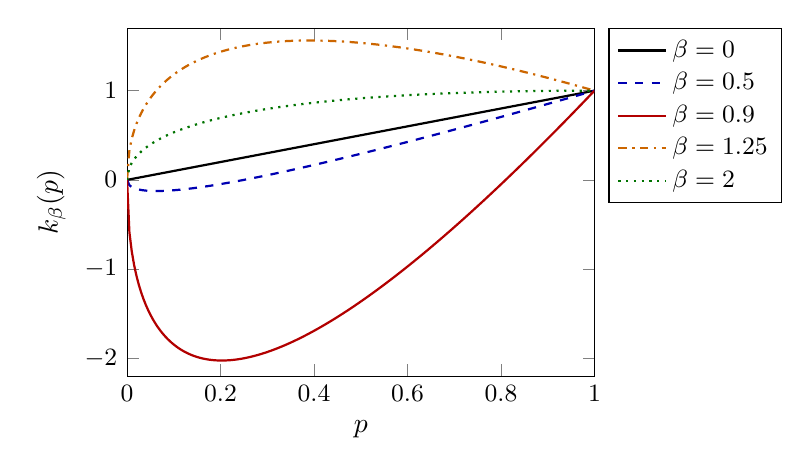
\begin{tikzpicture}
\begin{axis}[width=0.62\textwidth,height=6cm,xmin=0,xmax=1,ymin=-2.2,ymax=1.7,
  xlabel={$p$},ylabel={$k_\beta(p)$},tick label style={font=\small},samples=200,domain=0:1,
  legend pos=outer north east,legend style={font=\small,cells={anchor=west}}]
\addplot[thick,black] {x}; \addlegendentry{$\beta=0$}
\addplot[thick,blue!70!black,dashed] {(x-0.5*sqrt(x))/0.5}; \addlegendentry{$\beta=0.5$}
\addplot[thick,red!70!black] {(x-0.9*sqrt(x))/0.1}; \addlegendentry{$\beta=0.9$}
\addplot[thick,orange!80!black,dashdotted] {(x-1.25*sqrt(x))/(-0.25)}; \addlegendentry{$\beta=1.25$}
\addplot[thick,green!45!black,dotted] {(x-2*sqrt(x))/(-1)}; \addlegendentry{$\beta=2$}
\end{axis}
\end{tikzpicture}
\caption{The distortions $k_\beta$ of the associated family in Example~\ref{ex:family} ($h=\mathrm{id}$,
$g=\sqrt{\cdot}$). They are monotone for $\beta=0$ and $\beta=2$ and not monotone for $\beta\in(0,1)\cup(1,2)$.}
\label{fig:family}
\end{figure}

\begin{corollary}[Pooling at non-finite values]\label{cor:projpool}
Assume the axioms of Theorem~\ref{thm:A} and \ax{S}. Then for all comonotone $X,Y$,
\[
 \LR(X+Y)=\bracket{\rho(X)+\rho(Y)}{\Pi(X)+\Pi(Y)} .
\]
In terms of loss ratios and implied premiums alone:
\begin{center}\small
\begin{tabularx}{0.95\textwidth}{@{}>{\raggedright\arraybackslash}p{5.4cm}>{\raggedright\arraybackslash}X@{}}
\toprule
\textbf{Case} & \textbf{Pooled loss ratio}\\
\midrule
$X,Y\in D$, $\Pi(X)+\Pi(Y)\ne0$ & premium-weighted mean (\axCM)\\
$X,Y\in D$, premiums cancel & $\infty$ if $\LR(X)\ne\LR(Y)$; $\star$ if $\LR(X)=\LR(Y)$\\
$\Pi(X)=0$, $Y\in D$ & $\LR(Y)+\rho(X)/\Pi(Y)$, with $\rho(X)=\lim_{c\to0}c\,\LR(X+c)$\\
$\Pi(X)=\Pi(Y)=0$ & $\infty$ unless $\rho(X)=-\rho(Y)$, in which case $\star$\\
\bottomrule
\end{tabularx}
\end{center}
\end{corollary}

\begin{proof}
$\rho$ and $\Pi$ are comonotonic additive (Lemma~\ref{lem:comon}) and $\LR=\bracket{\rho}{\Pi}$ under \ax{S}
(Theorem~\ref{thm:A}). The table spells out $\bracket{\rho(X)+\rho(Y)}{\Pi(X)+\Pi(Y)}$, using $\rho=\Pi\,\LR$ on $D$
and Proposition~\ref{prop:readings}(c) for books with zero premium. If premiums cancel,
$\rho(X)+\rho(Y)=\Pi(X)(\LR(X)-\LR(Y))$. \qedhere
\end{proof}

The third row has a direct reading: a loss that is carried without premium adds its size, relative to the
premium base, to the loss ratio of the book it joins.

\begin{corollary}[Orderings, convexity and shape within the class]\label{cor:shape}
\begin{enumerate}[label=(\alph*)]
\item \emph{Endpoints.} $\rho$ is monotone iff $h$ is non-decreasing; $\rho$ is convex iff $h$ is concave
  \citep[Thm.~3]{www2020}; $\rho$ is coherent iff $h$ is concave and non-decreasing, in which case $\rho$ is a
  mixture of expected shortfalls $\mathrm{ES}_\alpha$ over levels $\alpha\in[0,1]$, with the convention
  $\mathrm{ES}_1:=\operatorname{ess\,sup}$ \citep{kusuoka2001,jst2006,folmerschied2016} and \citet[Thm.~5]{www2020b}; the endpoint is needed, for
  instance, for $h=\1_{(0,1]}$, which gives $\rho=\operatorname{ess\,sup}$. The same holds for $\Pi$ and $g$.
\item \emph{Ordering.} $\LR\le1$ on $\{\Pi>0\}$ iff $h\le g$.
\item \emph{Convex acceptance cones.} For $\beta\ne1$ let $A_\beta:=\{\rho\le\beta\Pi\}=\{I_{h-\beta g}\le0\}$.
  Then $A_\beta$ is convex iff $h-\beta g$ is concave, and all $A_\beta$, $\beta\in[0,\infty)\setminus\{1\}$, are
  convex iff $h$ is concave and $g$ is convex.
\item \emph{Quasi-convexity and quasi-concavity (sufficient conditions).}
  If $h$ is concave and $g$ is convex, then $\{\Pi>0\}$ is convex, $\LR\ge1$ there, and $\LR$ is quasi-convex on it.
  If, in Theorem~\ref{thm:B} with $g>0$, $h$ is convex and $g$ is concave, then $\LR\le1$ on $\Xp$ and $\LR$ is
  quasi-concave on $\Xp$. In particular the actuarial ratio $\E/C_g$ with $g$ concave is quasi-\emph{concave}.
\item \emph{Rigidity.} $\rho_\beta$ is convex for all $\beta\in[0,\infty)\setminus\{1\}$ iff $h=g$ and $g$ is concave.
\end{enumerate}
\end{corollary}

\begin{proof}
(a) The monotonicity criterion is in \citet{www2020}, see also \citet[Prop.~2]{www2020b}, and the
convexity criterion is \citet[Thm.~3]{www2020}.
(b) If $h\le g$ then $g-h\ge0$ with $(g-h)(1)=0$, so $I_{g-h}\ge0$ and $\LR\le1$ where $\Pi>0$. If $h(p)>g(p)$ for some $p$,
then $\LR(\1_A+c)=(h(p)+c)/(g(p)+c)>1$ for large $c$, where the premium $g(p)+c$ is positive.
(c) $I_{h-\beta g}$ has cash slope $1-\beta\ne0$, so all its sublevel sets are translates of $A_\beta$; hence
convexity of $A_\beta$ is quasi-convexity of $I_{h-\beta g}$, which is equivalent to concavity of $h-\beta g$
\citep[Thm.~3]{www2020}. Taking $\beta=0$ and $\beta\to\infty$ in $(h-\beta g)/\beta$ gives the second statement.
(d) If $h$ is concave and $g$ is convex then $I_g$ is concave, so $\{I_g>0\}$ is convex; $h\ge\mathrm{id}\ge g$, so
$\LR\ge1$; and for $\beta\ge1$ the set $\{I_h-\beta I_g\le0\}$ is convex because $h-\beta g$ is concave. If
$h$ is convex and $g$ concave, then $h\le\mathrm{id}\le g$, and $I_h-tI_g$ is concave for $t\ge0$, so
$\{\LR\ge t\}$ is convex; for $t<0$ the superlevel set is all of $\Xp$, since $I_h\ge0$ and $I_g>0$ on $\Xp$.
(e) Convexity of $\rho_\beta=I_{k_\beta}$ for $\beta<1$ means $h-\beta g$ concave, and for $\beta>1$ means
$h-\beta g$ convex. Letting $\beta\to1^\mp$ gives $h-g$ concave and convex, hence affine with zero endpoints, i.e.\
$h=g$; then $k_\beta=g$ and $\rho_\beta$ is convex iff $g$ is concave. The converse is clear. \qedhere
\end{proof}

In particular, the actuarial ratio $\E/C_g$ with $g$ concave is quasi-concave and not, in general, quasi-convex.

\begin{example}\label{ex:qc}
Let $A,B$ be disjoint with $P(A)=0.2$, $P(B)=0.3$, and $X_t=(1-t)\1_A+t\1_B$, $t\in[0,1]$. For
$\mathrm{ES}_{0.9}/\E$ (Example~\ref{ex:ES}), $\mathrm{ES}_{0.9}(X_t)=\max\{1-t,t\}$ and
$\LR(X_t)=\max\{1-t,t\}/(0.2+0.1t)$, which equals $5$ at $t=0$, $10/3$ at $t=1$ and $2$ at $t=\tfrac12$: the ratio
lies below the larger endpoint value, as quasi-convexity requires. For $\E/C_{\sqrt{\cdot}}$ the ratio equals
$\sqrt{0.2}\approx0.447$ at $t=0$, $\sqrt{0.3}\approx0.548$ at $t=1$ and $\sqrt{0.5}\approx0.707$ at $t=\tfrac12$: it lies
above the smaller endpoint value, as quasi-concavity requires (Figure~\ref{fig:qc}).
\end{example}

\begin{figure}[ht]
\centering
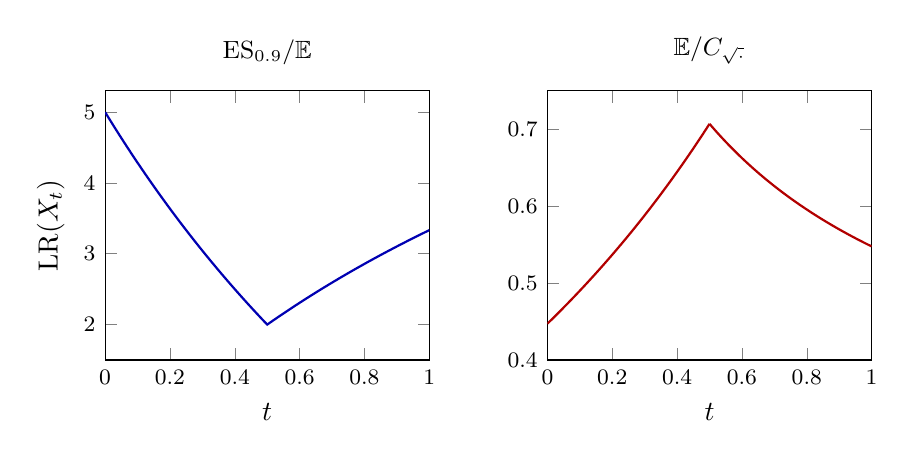
\begin{tikzpicture}
\begin{axis}[name=l,width=0.47\textwidth,height=5cm,xmin=0,xmax=1,ymin=1.5,ymax=5.3,xlabel={$t$},
  ylabel={$\LR(X_t)$},title={\small $\mathrm{ES}_{0.9}/\E$},tick label style={font=\footnotesize},samples=101,domain=0:1]
\addplot[thick,blue!70!black] {max(1-x,x)/(0.2+0.1*x)};
\end{axis}
\begin{axis}[at={(l.south east)},xshift=1.5cm,width=0.47\textwidth,height=5cm,xmin=0,xmax=1,ymin=0.4,ymax=0.75,
  xlabel={$t$},title={\small $\E/C_{\sqrt{\cdot}}$},tick label style={font=\footnotesize},samples=60]
\addplot[thick,red!70!black,domain=0:0.5] {(0.2+0.1*x)/(0.70711*x+0.44721*(1-2*x))};
\addplot[thick,red!70!black,domain=0.5:1] {(0.2+0.1*x)/(0.70711*(1-x)+0.54772*(2*x-1))};
\end{axis}
\end{tikzpicture}
\caption{Loss ratios along the segment $X_t=(1-t)\1_A+t\1_B$ of Example~\ref{ex:qc}: quasi-convex for
$\mathrm{ES}_{0.9}/\E$ (left) and quasi-concave for $\E/C_{\sqrt{\cdot}}$ (right).}\label{fig:qc}
\end{figure}

\begin{example}[Further special cases]
(1) \emph{Wang--Young--Panjer pairs} on nonnegative losses: Theorem~\ref{thm:C}.
(2) \emph{Coherent pairs}: $h,g$ concave non-decreasing; $\rho_\beta$ is a signed mixture of expected shortfalls.
(3) \emph{Actuarial ratio} $\E/C_g$, $h=\mathrm{id}$: Proposition~\ref{prop:unique} gives $g(p)=p/\LR(\1_A)$ for $P(A)=p$, so the
premium distortion is identified from the loss ratios of Bernoulli books.
(4) \emph{VaR-type pairs} are admissible in Theorem~\ref{thm:B}; $\rho_\beta$ is non-monotone near $\beta=1$; a
VaR-type premium $g=\1_{(a,1]}$ is excluded from Theorem~\ref{thm:C}, since $g>0$ fails.
(5) \emph{Gini-type ratios}: $\LR-1=I_{h-g}/I_g$ is a location-invariant signed Choquet ``variability'' divided by a
premium (compare \citealp{bfww2022}).
\end{example}

\section{Discussion and open problems}\label{sec:discussion}

\paragraph{Summary.}
A loss ratio carries its own premium and its own risk measure. The premium is the price point of the cash
line, the sure payment at which the book changes hands, and the risk measure is loss ratio times premium,
visible even where the ratio explodes as the residue of the singularity. With this reading, a single
substantive axiom, comonotone pooling at relative cost, together with law invariance and regularity of the
implied pair, characterizes the loss ratios that are ratios of two Choquet-type functionals. The
characterization is sharp, and the pair is unique. At the level of representations it is a transfer of the
theory of \citet{yaari1987}, \citet{schmeidler1986}, \citet{wyp1997} and \citet{www2020}; at the level of the
loss ratio it is new, and it comes with facts that have no single-functional counterpart: no non-trivial loss
ratio is monotone (Proposition~\ref{prop:F2}), the association holds exactly off $\{\rho=\Pi=0\}$ and is
signed (Corollary~\ref{cor:assoc}), and pooling extends consistently to books with infinite or indeterminate
loss ratios (Corollary~\ref{cor:projpool}).

\paragraph{Open problems.}
\begin{enumerate}[label=(\arabic*)]
\item \emph{Beyond comonotone pooling.} The most promising direction is to drop \axCM{} in favour of an axiom
  that allows diversification, so that the implied premium and risk measure are convex or subadditive rather
  than comonotonic additive. The implied premium and the implied risk measure are defined without \axCM{} only
  partly (the premium needs only \axP; the accounting reading of $\rho$ needs pooling with sure losses), and the
  resulting class, a ratio of Kusuoka-type functionals, has no characterization yet. Replacing comonotonic
  additivity by convexity leads to suprema of signed Choquet integrals \citep{liu2020}, so no single pair $(h,g)$
  and no uniqueness should be expected.
\item \emph{Weaker cardinal axioms.} Can \axCM{} be replaced by the mediant inequality plus a supplementary
  condition? The inequality implies additivity for comonotone pairs strictly on the same side of break-even, but
  not for pairs straddling $1$ or lying in the break-even set.
\item \emph{Order properties of $\LR$.} \axRM{} is monotonicity of the implied pair. Whether it is equivalent to a
  natural order property of $\LR$ is open; by Proposition~\ref{prop:F2} it cannot be pointwise monotonicity.
\item \emph{Loadings on sure losses.} We conjecture that an analogue of Theorem~\ref{thm:A} holds for ratios
  $\bracket{I_h}{\kappa I_g}$ with a known loading $\kappa>0$, which would admit constant loss ratios $\ne1$.
\item \emph{Quasi-convexity.} Necessity of the conditions in Corollary~\ref{cor:shape}(d) is open.
\item \emph{Actuarial domain.} Whether (A4) imposed only on pairs with $X,Y,X+Y\notin N_0$ suffices is open; a
  truncation-continuity (Greco-type) version of the signed tier on the cone is not known.
\item \emph{Unbounded losses.} Extensions to $L^p$ and Orlicz spaces via \citet{www2020b} are not treated.
\end{enumerate}

\section{Use of artificial intelligence}\label{sec:collab}

This paper also serves as a brief case study of the use of AI in mathematical research in actuarial science. This
section describes how AI was used and how the process was handled, and is meant to illustrate a standard for
reporting such use in a mathematical paper. The tools are identified in the declaration before the references. The section also describes how
the models acquire knowledge, the risks this entails for mathematical work, the guardrails used, the formal check
in Lean, and what has and has not been checked.

\subsection{Organization of the work}

The work used Claude (Anthropic) through the Claude desktop application in Cowork mode, which runs the assistant in
a sandboxed environment and can coordinate several AI agents in a workflow. AI agents worked on designated parts of
the project, under the author's direction. A main assistant organized the work and drafted and revised the
manuscript. A roundtable of six agents, five of them each assigned a strand of the literature and one acting as
chair, surveyed the axiomatic theory of premiums, risk measures and performance ratios and produced a synthesis. A
larger panel of agents covered ten literature strands, proposed candidate statements, ranked them by means of judge
agents, drafted proofs, and subjected the proofs to separate AI-assisted checking runs over several rounds. The
literature review was conducted by these AI assistants under the author's supervision: the author defined the
strands to be covered and the questions to be answered, and selected and framed the material presented in
Section~\ref{sec:lit}. Some agents were given the names of researchers as personas, to represent the
perspective of a literature strand; these were simulations, and the researchers concerned did not participate, were
not consulted and bear no responsibility for the content. The research questions, the choice of formulation and all
decisions on the content of the paper were made by the author.

Figures~\ref{fig:workflow} and~\ref{fig:panel} show the organization of the work. In Figure~\ref{fig:workflow}
the author assigns the task of each AI component and reviews its output. Figure~\ref{fig:panel} shows the internal pipeline of the panel, in which candidate statements and
proofs pass through ranking and repeated critical review before being returned to the author.
Figure~\ref{fig:panelpic} gives a schematic picture of the panel: the ten strand agents around a shared digest,
the proof bench of judge, prover and checking agents, and the author's place in the loop.

\begin{figure}[ht]
\centering
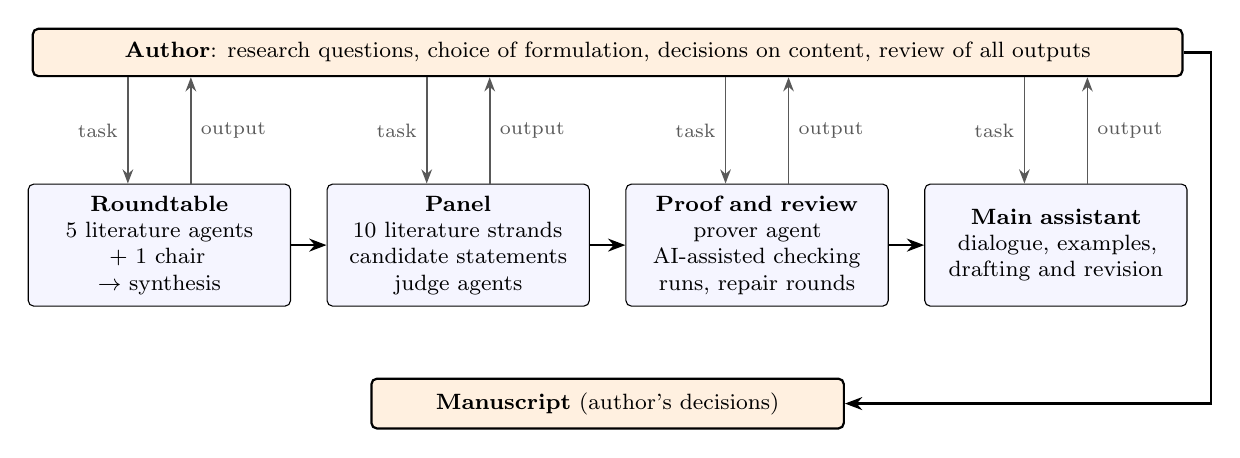
\begin{tikzpicture}[font=\footnotesize,
  box/.style={draw,rounded corners=2pt,align=center,inner sep=4pt,minimum height=1.55cm,text width=3.05cm,fill=blue!4},
  hum/.style={draw,thick,rounded corners=2pt,align=center,inner sep=5pt,fill=orange!12},
  arr/.style={-{Stealth[length=2.2mm]},thick},
  sarr/.style={-{Stealth[length=1.8mm]},semithick,gray!70!black}]
\node[box] (rt) {\textbf{Roundtable}\\ 5 literature agents\\ + 1 chair\\ $\to$ synthesis};
\node[box,right=0.45cm of rt] (pn) {\textbf{Panel}\\ 10 literature strands\\ candidate statements\\ judge agents};
\node[box,right=0.45cm of pn] (pr) {\textbf{Proof and review}\\ prover agent\\ AI-assisted checking\\ runs, repair rounds};
\node[box,right=0.45cm of pr] (ma) {\textbf{Main assistant}\\ dialogue, examples,\\ drafting and revision};
\draw[arr] (rt) -- (pn); \draw[arr] (pn) -- (pr); \draw[arr] (pr) -- (ma);
\node[hum,minimum width=14.6cm,above=1.35cm of $(pn.north)!0.5!(pr.north)$] (au)
  {\textbf{Author}: research questions, choice of formulation, decisions on content, review of all outputs};
\foreach \n in {rt,pn,pr,ma}{
  \draw[sarr] ([xshift=-4mm]au.south -| \n.north) -- node[left,font=\scriptsize]{task} ([xshift=-4mm]\n.north);
  \draw[sarr] ([xshift=4mm]\n.north) -- node[right,font=\scriptsize]{output} ([xshift=4mm]au.south -| \n.north);}
\node[hum,below=0.9cm of $(pn.south)!0.5!(pr.south)$,minimum width=6cm] (ms) {\textbf{Manuscript} (author's decisions)};
\draw[arr] (au.east) -- ++(0.35,0) |- (ms.east);
\end{tikzpicture}
\caption{Organization of the work. The author assigns tasks to each AI component and reviews every output; the
manuscript reflects the author's decisions. The stages were used in the order shown, with returns to earlier
stages when the author redirected the work.}\label{fig:workflow}
\end{figure}

\begin{figure}[ht]
\centering
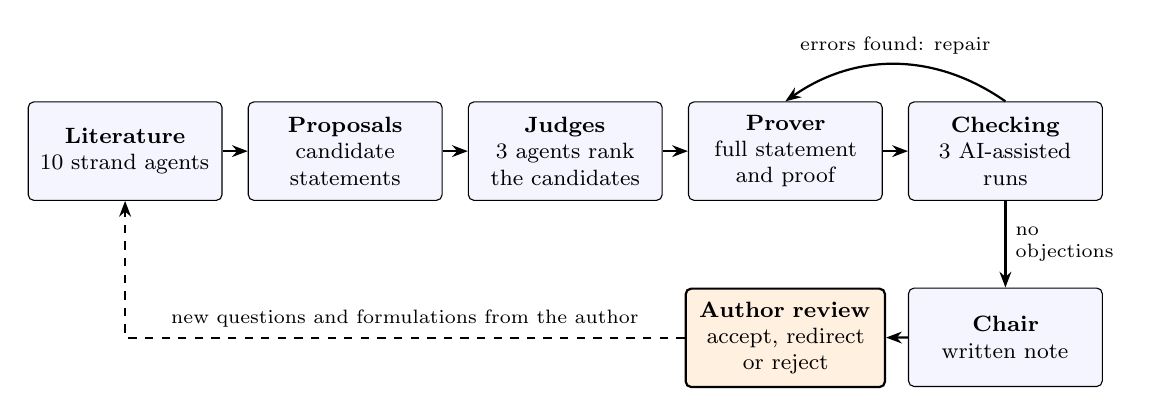
\begin{tikzpicture}[font=\footnotesize,
  st/.style={draw,rounded corners=2pt,align=center,inner sep=3pt,minimum height=1.25cm,text width=2.25cm,fill=blue!4},
  hum/.style={draw,thick,rounded corners=2pt,align=center,inner sep=4pt,text width=2.25cm,minimum height=1.25cm,fill=orange!12},
  arr/.style={-{Stealth[length=2mm]},thick}]
\node[st] (lit) {\textbf{Literature}\\ 10 strand agents};
\node[st,right=0.32cm of lit] (prop) {\textbf{Proposals}\\ candidate\\ statements};
\node[st,right=0.32cm of prop] (jud) {\textbf{Judges}\\ 3 agents rank\\ the candidates};
\node[st,right=0.32cm of jud] (prv) {\textbf{Prover}\\ full statement\\ and proof};
\node[st,right=0.32cm of prv] (chk) {\textbf{Checking}\\ 3 AI-assisted\\ runs};
\node[st,below=1.1cm of chk] (cha) {\textbf{Chair}\\ written note};
\node[hum,below=1.1cm of prv] (aut) {\textbf{Author review}\\ accept, redirect\\ or reject};
\draw[arr] (lit) -- (prop); \draw[arr] (prop) -- (jud); \draw[arr] (jud) -- (prv); \draw[arr] (prv) -- (chk);
\draw[arr] (chk.north) to[bend right=35] node[above,font=\scriptsize]{errors found: repair} (prv.north);
\draw[arr] (chk.south) -- node[right,font=\scriptsize,align=left]{no\\ objections} (cha.north);
\draw[arr] (cha) -- (aut);
\draw[arr,dashed] (aut.west) -- node[above,font=\scriptsize]{new questions and formulations from the author} (aut.west -| lit.south) -- (lit.south);
\end{tikzpicture}
\caption{Pipeline of the panel. Literature agents survey their strands; proposal agents formulate candidate
statements, which judge agents rank. A prover agent drafts a full statement and proof, which separate AI-assisted
checking runs examine; reported errors are sent back for repair over several rounds. A chair agent writes up the
result for the author, who accepts it, redirects the work or rejects it. Agreement among checking runs does not
establish correctness.}\label{fig:panel}
\end{figure}

\begin{figure}[ht]
\centering
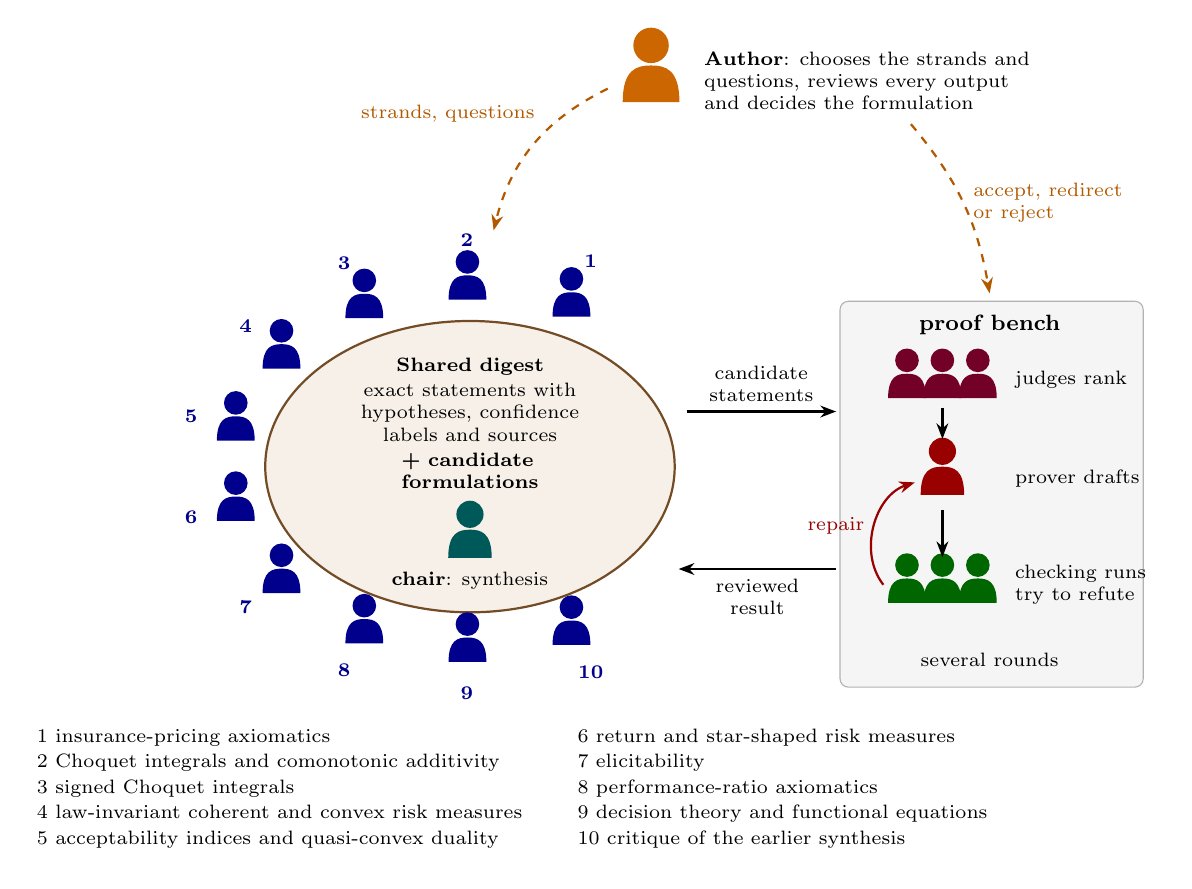
\begin{tikzpicture}[font=\scriptsize,
  person/.pic={
    \fill[pic actions] (0,0.30) circle (0.15);
    \fill[pic actions] (-0.24,-0.18) .. controls (-0.24,0.10) and (-0.12,0.13) .. (0,0.13)
                        .. controls (0.12,0.13) and (0.24,0.10) .. (0.24,-0.18) -- cycle;},
  lab/.style={align=center,text width=2.0cm,inner sep=1pt},
  arr/.style={-{Stealth[length=2mm]},thick},
  darr/.style={-{Stealth[length=2mm]},thick,dashed,orange!70!black}]
% table
\fill[brown!12] (0,0) ellipse (2.6 and 1.85);
\draw[brown!60!black,thick] (0,0) ellipse (2.6 and 1.85);
\node[align=center,text width=3.4cm] at (0,0.55) {\textbf{Shared digest}\\[1pt] exact statements with\\ hypotheses, confidence\\ labels and sources\\[1pt] \textbf{+ candidate formulations}};
\pic[fill=teal!70!black,scale=1.15] at (0,-0.95) {person};
\node at (0,-1.45) {\textbf{chair}: synthesis};
% ten strand agents
\foreach \ang [count=\k] in {65.0,90.6,116.1,141.7,167.2,192.8,218.3,243.9,269.4,295.0}{
  \pgfmathsetmacro{\px}{3.05*cos(\ang)} \pgfmathsetmacro{\py}{2.3*sin(\ang)}
  \pic[fill=blue!55!black] at (\px,\py) {person};
  \node[font=\scriptsize\bfseries,blue!55!black] at ($(\px,\py)+(\ang:0.58)$) {\k};
}
% proof bench on the right
\begin{scope}[xshift=6.0cm,yshift=-0.2cm]
  \draw[rounded corners=3pt,fill=gray!8,draw=gray!60] (-1.3,-2.6) rectangle (2.55,2.3);
  \node[font=\footnotesize\bfseries] at (0.6,2.0) {proof bench};
  \foreach \y in {0,1,2} {\pic[fill=purple!60!black] at (-0.45+0.45*\y,1.25) {person};}
  \node[anchor=west] at (0.8,1.3) {judges rank};
  \pic[fill=red!60!black,scale=1.15] at (0,0.05) {person};
  \node[anchor=west] at (0.8,0.05) {prover drafts};
  \foreach \y in {0,1,2} {\pic[fill=green!40!black] at (-0.45+0.45*\y,-1.35) {person};}
  \node[anchor=west,align=left] at (0.8,-1.3) {checking runs\\ try to refute};
  \draw[arr] (0,0.95) -- (0,0.55);
  \draw[arr] (0,-0.35) -- (0,-0.95);
  \draw[arr,red!60!black] (-0.75,-1.3) to[bend left=55] node[left]{repair} (-0.35,0.0);
  \node at (0.6,-2.25) {several rounds};
\end{scope}
\draw[arr] (2.75,0.7) -- node[above,align=center]{candidate\\ statements} (4.65,0.7);
\draw[arr] (4.65,-1.3) -- node[below,align=center]{reviewed\\ result} (2.65,-1.3);
% author
\pic[fill=orange!80!black,scale=1.5] at (2.3,4.9) {person};
\node[align=left,anchor=west] at (2.85,4.9) {\textbf{Author}: chooses the strands and\\ questions, reviews every output\\ and decides the formulation};
\draw[darr] (1.75,4.8) to[bend right=25] node[above left,pos=0.4]{strands, questions} (0.3,3.0);
\draw[darr] (5.6,4.35) to[bend left=15] node[right,pos=0.5,align=left]{accept, redirect\\ or reject} (6.6,2.2);
% key
\node[anchor=north,align=left,text width=14.2cm,font=\scriptsize] at (1.6,-3.15) {%
\begin{tabular}{@{}l@{\hspace{2.5em}}l@{}}
1 insurance-pricing axiomatics & 6 return and star-shaped risk measures\\
2 Choquet integrals and comonotonic additivity & 7 elicitability\\
3 signed Choquet integrals & 8 performance-ratio axiomatics\\
4 law-invariant coherent and convex risk measures & 9 decision theory and functional equations\\
5 acceptability indices and quasi-convex duality & 10 critique of the earlier synthesis
\end{tabular}};
\end{tikzpicture}
\caption{The panel at work. Ten literature agents (numbered as in the key), each assigned a strand by the author, write exact statements
into a shared digest, which together with the candidate formulations forms the knowledge base read in full by the
later agents; a chair agent synthesizes. Candidate statements pass to the proof bench, where judge agents rank them,
a prover agent drafts proofs and separate checking runs try to refute them, with errors returned for repair. The
author sets the strands and questions and accepts, redirects or rejects each result. The icons are schematic: the
agents are separate runs of a language model.}\label{fig:panelpic}
\end{figure}


AI assisted with the following tasks:
\begin{itemize}[nosep]
\item literature exploration;
\item formulation of mathematical statements and drafting of proofs;
\item construction of counterexamples and examples;
\item manuscript drafting and revision.
\end{itemize}


\subsection{How the knowledge base for this paper was assembled}

The agents draw on two kinds of knowledge: what their underlying models learned in training, which can be
recalled only approximately, and documents read into their working context during the task. In this project the
second kind was organized as follows.

The five strands of the roundtable were identified by the author: premium principles and capital allocation;
conic finance and performance ratios; coherent risk measures and acceptance sets; axiomatic risk measures and
elicitability; and the extended-loss-ratio framework with its association. Its synthesis served as the starting
point of the panel.

The panel divided the literature into ten strands: insurance-pricing axiomatics; Choquet integrals and comonotonic
additivity; signed Choquet integrals; law-invariant coherent and convex risk measures; acceptability indices and
quasi-convex duality; return and star-shaped risk measures; elicitability; performance-ratio axiomatics; decision
theory and functional equations; and a critique of the earlier synthesis. Each strand agent returned exact
statements of if-and-only-if theorems with their hypotheses, a confidence label (high, medium or low) and a note
on its source. For example, the signed representation results of
\citet{cmmm2012,cmmm2015} were taken from their working paper versions.

There was no separate retrieval index. Instead, the strand reports were merged into a written digest of about
415{,}000 characters, which, together with the ten candidate formulations (about 245{,}000 characters), formed the
shared knowledge base of the later stages: the judge and prover agents were instructed to read these files in full
before working, and Section~\ref{sec:lit} was written from the digest. The confidence labels therefore
travelled with each statement into the stages that used it.

In addition, the author used Gemini (Google) to prepare summaries of the key works cited in
Section~\ref{sec:lit}: \citet{gerber1974}, \citet{yaari1987} and \citet{wyp1997} on premium principles;
\citet{msm1994}, \citet{cmmm2012,cmmm2015} and \citet{www2020} on signed Choquet integrals; \citet{adeh1999} and
\citet{kusuoka2001} on coherent risk measures; and \citet{chernymadan2009}, \citet{chew1983} and \citet{dekel1986} on
performance ratios and ratio representations. Each summary stated the core results of the work and their role in
this paper. The descriptions in Section~\ref{sec:lit} and the uses of these works in Sections~\ref{sec:axioms},
\ref{sec:results}, \ref{sec:necessity} and~\ref{sec:consequences} were compared with these summaries; no
discrepancy was found, and three descriptions in Section~\ref{sec:lit} were made more precise. Since the summaries
are themselves AI output, this comparison is a consistency check, not a check against the original publications.

Later, the author supplied author versions of three cited papers: \citet{www2020} (working paper of June 2019),
\citet{www2020b} (version of May 2020, with a correction of May 2023) and \citet{hlw2025} (version of June 2024).
The statements taken from them were checked against these versions: the definition of $I_h$, the
characterization theorem used in the representation step and the convexity theorem of \citet{www2020}; the
monotonicity criterion and Lipschitz bound, which are also stated there; the extension to general spaces, the
convention $\mathrm{ES}_1=\operatorname{ess\,sup}$ and the mixture representation of \citet{www2020b}; and the
axioms and the two characterization theorems of \citet{hlw2025}. No discrepancy was found. Lemma numbers that
could differ between these versions and the published articles were removed, and the description of
\citet{hlw2025} in Section~\ref{sec:lit} was rewritten from the paper.

\subsection{Hallucinations and semantic errors encountered}

\emph{Statements about the literature.} The main risk of hallucination concerned the exact hypotheses, conclusions
and numbering of cited results. Two entries of the digest disagreed on whether the mixing measure in the Kusuoka
representation includes an atom at the endpoint; the paper therefore states the mixture over $[0,1]$ with an
explicit convention (Corollary~\ref{cor:shape}(a)) and cites the representation without theorem numbers. For the
same reason, the representation step used in the proofs is not taken from the literature but reproved
(Lemmas~\ref{lem:cashlip}--\ref{lem:rep}).

\emph{Errors in mathematical content.} Table~\ref{tab:errors} lists the errors in AI-generated mathematics that were
found during the project. Most are semantic: the statement proved, or claimed, differed from the statement
intended, typically at a degenerate case (zero premium, the break-even set, the labels $\infty$ and $\star$) or in
the scope of a claim.

\begin{table}[ht]
\centering\footnotesize
\begin{tabularx}{\textwidth}{@{}>{\raggedright\arraybackslash}X>{\raggedright\arraybackslash}p{2.6cm}>{\raggedright\arraybackslash}X@{}}
\toprule
\textbf{Error} & \textbf{Found by} & \textbf{Resolution}\\
\midrule
$\E/C_g$ with concave $g$ claimed quasi-convex (early synthesis) & panel agents & quasi-concave; Cor.~\ref{cor:shape}(d)\\
quasi-convexity stated as an if-and-only-if in four candidate formulations & judge agent ($h=t$, $g=\sqrt t$, $\beta=2$) & only sufficient conditions kept\\
candidate route via Sincov and Cauchy equations & judge agent (continuous $h$ not of bounded variation) & route abandoned\\
main argument claimed to apply verbatim when $(\rho,\Pi)$ is only assumed to exist & checking run & separate argument given\\
association claimed to hold exactly on the finite domain & checking run & holds off $\{\rho=\Pi=0\}$; Cor.~\ref{cor:assoc}(a)\\
``$h-g$ concave'' as a sufficient condition for quasi-convexity & main assistant, during rewriting & $h$ concave, $g$ convex\\
converse of Theorem~\ref{thm:A} failed for \axLI{} (labels unconstrained) & checking run & \axLI{} compares finite values only\\
claimed equivalence with the cash-line formulation & checking run & convention \ax{S} added; Remark~\ref{rem:oldCP}\\
regularity axioms undefined for two counterexamples & checking run & \axRC, \axRM{} stated for $\Pi$ and $\rho_D$\\
uniqueness of the extension in Prop.~\ref{prop:bridge} & review with ChatGPT & unique up to labels, unique under \ax{S}\\
independence claimed for (A0) and (A1) & review with ChatGPT & treated as illustrations; Sec.~\ref{sec:necessity}\\
mixture of expected shortfalls missing the endpoint & review with ChatGPT & $\mathrm{ES}_1:=\operatorname{ess\,sup}$; Cor.~\ref{cor:shape}(a)\\
\bottomrule
\end{tabularx}
\caption{Errors in AI-generated mathematics found during the project, and their resolution.}\label{tab:errors}
\end{table}

\subsection{Guardrails applied in this project}

\begin{itemize}[nosep]
\item \emph{Labels on knowledge.} Every literature statement in the digest carried a confidence label and a note on
  its source, as described above.
\item \emph{Independent summaries.} Summaries of the key cited works prepared with Gemini were compared with their
  descriptions and uses in the paper.
\item \emph{Self-contained proofs.} Results whose exact statements were uncertain are reproved; in particular the
  representation of comonotonic additive functionals, for which the proof cites \citet[Thm.~1]{www2020}, is
  reproved in Lemmas~\ref{lem:cashlip}--\ref{lem:rep}.
\item \emph{Adversarial checking.} The three checking runs on the panel's proofs were instructed to refute; one tested
  the degenerate case $\LR\equiv1$ with a premium that is not comonotonic additive, and two recomputed the numbers in
  the counterexamples. The restructured formulation of Sections~\ref{sec:axioms}--\ref{sec:proofs} was given to a
  further checking run with instructions to look for circularity and for the cases $\Pi(X)=0$, break-even books,
  $\LR\equiv1$ and $c=0$.
\item \emph{Repair loop.} Reported gaps were returned to the prover agent; the panel's proofs went through two
  repair rounds before the final checking round.
\item \emph{Counterexamples.} Each axiom other than \axP{} is tested against an explicit loss ratio
  (Section~\ref{sec:necessity}).
\item \emph{Recomputation.} The values in Examples~\ref{ex:PH}, \ref{ex:ES}, \ref{ex:qc} and in the counterexamples
  were recomputed by script, and the monotonicity range in Example~\ref{ex:family} was confirmed on a grid.
\item \emph{Formal checking.} The loss-ratio-specific steps were formalized in Lean and compiled; see
  Section~\ref{sec:collab-lean}.
\item \emph{A second system.} The review with ChatGPT, a model from a different provider, found three of the errors in
  Table~\ref{tab:errors} that the earlier checks had missed.
\end{itemize}

\subsection{What the prover produced and what was formally checked}

The ``prover'' of Figure~\ref{fig:panel} is a language-model agent that writes proofs in ordinary mathematical
language; it is not a formal theorem prover. In this project it drafted the first complete if-and-only-if theorem,
in a formulation based on an assumed cash-line axiom, with proofs of the results that are now
Theorems~\ref{thm:A}, \ref{thm:B}, \ref{thm:A0}, \ref{thm:C} and~\ref{thm:Cp} and of the appendix lemmas; the final
checking round of these proofs returned two reports without objections and one report of gaps in side claims, which
were repaired. The present formulation through the implied premium and risk measure
(Lemmas~\ref{lem:premium}--\ref{lem:LI} and Proposition~\ref{prop:readings}) was drafted afterwards by the main
assistant and checked by one further run, whose findings appear in Table~\ref{tab:errors}.

The loss-ratio-specific steps were also checked formally in Lean (Section~\ref{sec:collab-lean}).

\subsection{Formal checking in Lean}\label{sec:collab-lean}

\subsubsection*{Lean and what a formal check establishes}

Lean~4 \citep{demoura2021} is an interactive proof assistant: a programming language in which definitions,
statements and proofs are written in a formal language based on dependent type theory, and in which every proof is
checked by a small trusted program, the kernel. A proof may be written step by step or with the help of tactics,
procedures that search for parts of a proof automatically, but whatever a tactic produces is checked again by the
kernel. Mathlib \citep{mathlib2020} is the community library of formalized mathematics for Lean; it supplies the
real numbers, groups, limits and the other notions used below.

Two features of Lean are used to state precisely what has been checked. A proof can be left unfinished by writing
\texttt{sorry}, which Lean accepts with a warning; a finished development contains none. The command
\texttt{\#print axioms} lists the foundational axioms on which a theorem depends; ordinary classical mathematics in
Lean uses exactly three of them, \texttt{propext} (propositional extensionality), \texttt{Classical.choice} (the
axiom of choice) and \texttt{Quot.sound} (soundness of quotients), and an unfinished proof shows up in this list as
\texttt{sorryAx}.

A successful check establishes that the formal statements follow from the formal definitions. It does not
establish that the formal definitions and statements say what the paper says, which must be checked by a human
reader, and it says nothing about results that enter as hypotheses or are not formalized.

For this paper a formal check is useful for three reasons. First, the proofs were drafted with AI assistance, and
the errors recorded in Table~\ref{tab:errors} show that such drafts can contain steps that read well and are wrong;
the kernel does not depend on how a proof was produced. Second, the steps that are specific to loss ratios
(Lemmas~\ref{lem:premium}--\ref{lem:LI}) are elementary but delicate, with case distinctions at $\Pi(X)=0$, at
break-even books and at the price point, which is where informal checking is most likely to miss a case. Third,
formalization forces the hypotheses to be stated exactly, and here it shows that those steps use only a few
algebraic properties of comonotonicity and equality in law (see ``What was formalized'' below).

\subsubsection*{What was formalized}\label{sec:lean-scope}

The formalization works in an abstract setting. Positions form an additive commutative group $\Xp$ with an additive
embedding $c\mapsto\mathrm{const}(c)$ of the sure losses, a relation ``comonotone'' under which every position is
comonotone with every constant and which is preserved when both positions are shifted by constants, and a relation
``equal in law'' preserved by a common cash shift. A loss ratio is a map from $\Xp$ to $\R\cup\{\mathtt{none}\}$,
where \texttt{none} stands for a non-finite value, so that the labels $\infty$ and $\star$ are identified as in
\axLI. The axioms read as follows; \texttt{prem} is the implied premium and \texttt{rhoD} is $\Pi\cdot\LR$.

{\small
\begin{verbatim}
def AxP : Prop := ∀ x : X, ∃! c : ℝ, LR (x + S.const c) = none
def AxN : Prop := ∀ c : ℝ, c ≠ 0 → LR (S.const c) = some 1
def AxLI : Prop := ∀ x y : X, S.eqd x y → LR x = LR y
def AxCM (hP : AxP S LR) : Prop :=
  ∀ x y : X, S.comon x y → LR x ≠ none → LR y ≠ none →
    prem hP x + prem hP y ≠ 0 →
    LR (x + y) = some ((rhoD hP x + rhoD hP y) / (prem hP x + prem hP y))
\end{verbatim}
}

These coincide with Axioms~\ref{ax:P}, \ref{ax:N}, \ref{ax:CM} and~\ref{ax:LI}. The file has about 500 lines with
10 definitions and 26 lemmas and theorems. Table~\ref{tab:lean} lists the results of the paper that are formalized.

\begin{table}[ht]
\centering\small
\begin{tabular}{@{}ll@{}}
\toprule
\textbf{Result in the paper} & \textbf{Lean name}\\
\midrule
Implied premium, uniqueness and cash additivity (Lemma~\ref{lem:premium}) & \texttt{prem}, \texttt{prem\_shift}, \texttt{prem\_const}\\
Implied risk measure and cash additivity (Lemma~\ref{lem:implied}) & \texttt{rho}, \texttt{rho\_cash}\\
Möbius form and residue (Proposition~\ref{prop:readings}(a)--(c)) & \texttt{mobius}, \texttt{rho\_eq}, \texttt{residue}\\
Comonotonic additivity, also on the break-even set (Lemma~\ref{lem:comon}) & \texttt{comon\_additive}\\
Law invariance of the implied pair (Lemma~\ref{lem:LI}) & \texttt{LI\_transfer}\\
Converse construction and uniqueness of the pair & \texttt{converse}, \texttt{unique\_pair}\\
Association (Corollary~\ref{cor:assoc}(a)) & \texttt{association}\\
Pooling at non-finite values (Corollary~\ref{cor:projpool}) & \texttt{pooling\_extended}\\
Algebraic core of Proposition~\ref{prop:F2} & \texttt{no\_monotone\_core}\\
Theorem~\ref{thm:A}, given the representation step & \texttt{main\_conditional}\\
\bottomrule
\end{tabular}
\caption{Results formalized in Lean.}\label{tab:lean}
\end{table}

The theorem \texttt{main\_conditional} takes the representation step as a hypothesis: any cash-additive,
comonotonic additive, law-invariant and regular functional is of the required form \citep[Thm.~1]{www2020}. From
\axP, \axN, \axCM{} and \axLI{} it derives that the implied premium and the implied risk measure satisfy the
hypotheses of that step and that $\LR=\bracket{\rho}{\Pi}$ everywhere. Not formalized are the representation step
itself (Lemmas~\ref{lem:cashlip}--\ref{lem:rep}), which would require a theory of Choquet integrals that Mathlib does not
provide, the fact that $L^\infty$ with comonotonicity and equality in law is an instance of
the abstract setting, the layer formula, and the examples and counterexamples.

\subsubsection*{How the check was carried out}

The Lean file was written by the main assistant. Lean could not be installed in the assistant's cloud workspace,
whose network policy blocks the servers that distribute Lean, so the file was compiled on the author's computer.
The author installed Lean and created the project; the assistant read the build output from the project folder
through the link between the Claude desktop application and the author's computer, wrote corrected versions of the
file into the same folder, and the author ran the next build (Figure~\ref{fig:leanloop}).

\begin{figure}[ht]
\centering
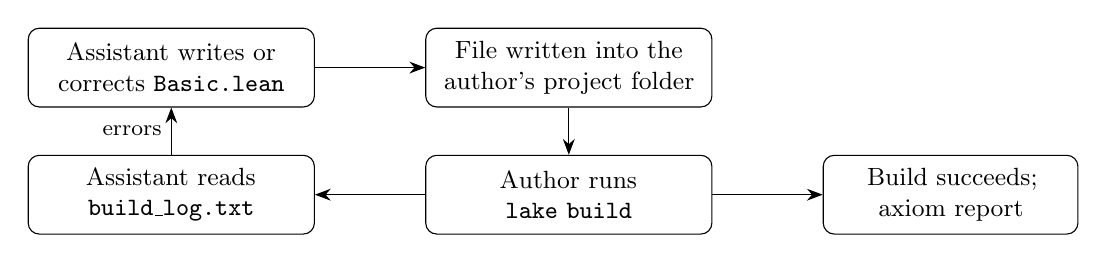
\begin{tikzpicture}[node distance=6mm and 14mm,
  box/.style={draw,rounded corners,align=center,font=\small,minimum height=10mm,text width=34mm},
  >={Stealth[length=2mm]}]
\node[box] (a) {Assistant writes or\\corrects \texttt{Basic.lean}};
\node[box,right=of a] (b) {File written into the\\author's project folder};
\node[box,below=of b] (c) {Author runs\\\texttt{lake build}};
\node[box,left=of c] (d) {Assistant reads\\\texttt{build\_log.txt}};
\draw[->] (a) -- (b);
\draw[->] (b) -- (c);
\draw[->] (c) -- (d);
\draw[->] (d) -- node[left,font=\footnotesize,align=center]{errors}(a);
\node[box,right=of c,text width=30mm] (e) {Build succeeds;\\axiom report};
\draw[->] (c) -- (e);
\end{tikzpicture}
\caption{The build-and-repair loop used for the Lean check.}\label{fig:leanloop}
\end{figure}

Table~\ref{tab:leantime} gives the timeline. Times are in UTC and are taken from the session records and from the
modification times of the files in the project folder.

\begin{table}[ht]
\centering\small
\begin{tabular}{@{}>{\raggedright\arraybackslash}p{3.3cm}>{\raggedright\arraybackslash}p{11.0cm}@{}}
\toprule
\textbf{Time (UTC)} & \textbf{Step}\\
\midrule
21 Oct, 21:38 & The assistant writes a first Lean file for the results in Table~\ref{tab:lean}; it cannot be compiled
  in the cloud workspace.\\
24 Oct, 17:08 & The author asks how a formal proof check can be used; the assistant describes what is feasible
  (the loss-ratio steps), what is hard (the representation step) and how to install Lean.\\
24 Oct, 17:26--17:31 & The author installs the Lean extension for the code editor and the Lean toolchain manager.\\
24 Oct, 17:35--17:37 & The author creates the project \texttt{loss\_ratio\_lean} with Mathlib; Lean and Mathlib
  version~4.36.0-rc1; the precompiled Mathlib files are downloaded.\\
24 Oct, 17:38--17:39 & The assistant inspects the project configuration, confirms that it is complete, and places
  the Lean file in it, replacing the template placeholder.\\
25 Oct, 12:47--12:53 & First attempt to build: the command \texttt{lake} is not found, because the toolchain had not
  been added to the terminal's search path; fixed by loading the toolchain environment.\\
25 Oct, 12:55 & Build 1: four errors, none in a definition or statement. One proof stopped one algebraic step short;
  in three proofs Lean's simplifier rewrote $\mathrm{const}(-c)$ as $-\mathrm{const}(c)$, so that cash additivity
  no longer applied.\\
25 Oct, 12:57 & The assistant writes a corrected file and appends \texttt{\#print axioms} for ten main theorems.\\
25 Oct, 13:04 & Build 2: one error, in the converse construction, where the goal was displayed in an unexpanded
  form. The axiom report shows the three standard axioms for nine theorems and \texttt{sorryAx} for the converse.\\
25 Oct, 13:05 & The assistant adds one line that states the goal explicitly.\\
25 Oct, 13:08 & Build 3 succeeds. All ten theorems depend only on the three standard axioms.\\
25 Oct, 13:09 & The assistant compares the Lean definitions of \axP, \axN, \axCM{} and \axLI{} and the theorem
  statements with Section~\ref{sec:axioms}.\\
25 Oct, 13:37 & At the author's request, the project's own build output is deleted and the file is rebuilt from
  scratch: success in 8.8\,s, with the same axiom report.\\
\bottomrule
\end{tabular}
\caption{Timeline of the Lean check.}\label{tab:leantime}
\end{table}

\subsubsection*{Checks performed}

The following checks were made to ensure that the outcome is what is reported.

\begin{itemize}[nosep]
\item \emph{No change to statements during repair.} The corrections after builds 1 and 2 changed proof steps only;
  no definition and no theorem statement was altered.
\item \emph{No unfinished proofs.} The final file contains no \texttt{sorry}, no \texttt{admit} and no added
  \texttt{axiom}.
\item \emph{Axiom report.} \texttt{\#print axioms} for each of the ten theorems in Table~\ref{tab:lean} lists only
  \texttt{propext}, \texttt{Classical.choice} and \texttt{Quot.sound}.
\item \emph{Clean rebuild.} The final build started from an empty build directory, so its result does not rely on
  cached output.
\item \emph{Identity of the file.} The file compiled in the final build was compared with the file reported here and
  found identical.
\item \emph{Fidelity of statements.} The formal axioms and theorem statements were compared with the paper by the
  assistant; this comparison is to be repeated by the author before the code is released.
\end{itemize}

The remaining warnings concern style and the use of renamed library lemmas; they do not affect correctness. The Lean
source and the build log are available in the repository
\url{https://github.com/hirbod-assa/loss-ratio-lean}, which contains the Lean project (Lean and Mathlib
version~4.36.0-rc1) together with instructions for rebuilding it with \texttt{lake build}.


\subsection{Verification status}\label{sec:collab-status}

The proofs have undergone AI-assisted critical review. Such review is fallible and does not
constitute formal verification; this applies equally to the informal review with ChatGPT. No claim of
machine-checked correctness is made beyond the results formalized in Lean, in the abstract setting and with the
hypothesis described in Section~\ref{sec:collab-lean}. Independent human review of all proofs, and journal peer review, have not yet taken
place, and apart from the three papers named above the references have not yet been checked against the original
publications.


\appendix
\section{Proof of Theorem~\ref{thm:A0} (no law invariance)}\label{app:A0}


Lemmas~\ref{lem:premium}, \ref{lem:implied}, \ref{lem:comon} and~\ref{lem:cashlip} do not use \axLI. Put
$\nu_1(A):=\rho(\1_A)$ and $\nu_2(A):=\Pi(\1_A)$. They are null-invariant, because $\rho$ and $\Pi$ act on
almost-sure classes, normalized by $\rho(1)=\Pi(1)=1$, and the layer formula \eqref{eq:layer} holds with
$\nu_i(C_j)$ in place of $h(P(C_j))$, for every chain $C_1\supset\dots\supset C_m$.

\emph{Bounded variation.} Given a chain $\emptyset=A_0\subset\dots\subset A_n=\Omega$, run the proof of
Lemma~\ref{lem:bv} with $I_j:=A_j\setminus A_{j-1}$; then $\{W\ge2(n-j)\}=A_j$, and one obtains
$\|\nu_1\|_{bv}\le2L$. Under \axRM, $\nu_1$ is monotone, i.e.\ a capacity.

\emph{Jordan decomposition of a game.} For $\nu\in\mathcal V$ let $\nu^+(A):=\sup\sum_j(\nu(A_j)-\nu(A_{j-1}))^+$
over chains from $\emptyset$ to $A$, and $\nu^-:=\nu^+-\nu$.
For $A\subset B$, appending $B$ to a chain for $A$ gives $\nu^+(B)\ge\nu^+(A)+(\nu(B)-\nu(A))^+$. Hence $\nu^+$ is
non-decreasing, and $\nu^-(B)-\nu^-(A)\ge(\nu(B)-\nu(A))^+-(\nu(B)-\nu(A))\ge0$, so $\nu^-$ is non-decreasing.
Moreover $\nu^+(A)\le\|\nu\|_{bv}$ (append $\Omega$), and null-invariance passes to $\nu^\pm$ (if $P(A\triangle A')=0$,
map $A_j\mapsto A_j\cap A'$ for $j<n$ and $A_n\mapsto A'$, which preserves all $\nu$-values).

\emph{Representation.} $C_{\nu^\pm}$ (with the correction term by $\nu^\pm(\Omega)$) is monotone with cash slope
$\nu^\pm(\Omega)$, hence Lipschitz, and $C_\nu=C_{\nu^+}-C_{\nu^-}$ by linearity in $\nu$. Now $\rho$ and
$C_{\nu_1}$ are Lipschitz and agree on simple positions by \eqref{eq:layer}, so $\rho=C_{\nu_1}$; likewise
$\Pi=C_{\nu_2}$.

\emph{Converse and uniqueness.} As in the proof of Theorems~\ref{thm:A} and~\ref{thm:B}, with $\nu$ in place of
$h\circ P$; null-invariance makes $C_\nu$ well defined on almost-sure classes and makes almost-sure nestedness
sufficient. Uniqueness follows because $\Pi(\1_A)$ is minus the price point of $\1_A$ and $\rho(\1_A)$ is given by
Proposition~\ref{prop:readings}(b).

\emph{Law invariance.} If \axLI{} holds, Lemma~\ref{lem:LI} makes $\nu_i(A)$ a function of $P(A)$ alone, so
$\nu_i=k_i\circ P$; since the space is atomless, $\|k\circ P\|_{bv}=\TV(k)$, so $k_i\in\Hset_1$. Conversely
$k\circ P$ gives a law-invariant functional. \qed

\section{Proofs for the actuarial domain}\label{app:C}


\begin{proof}[Proof of Lemma~\ref{lem:halfline}]
$a/b=\LR_0(X)\ne1$, so $a\ne b$. \emph{Uniqueness.} If $(a+c)(b'+c)=(a'+c)(b+c)$ for all $c\ge0$, comparing
coefficients gives $a+b'=a'+b$ and $ab'=a'b$; writing $a'=a+t$, $b'=b+t$ gives $t(a-b)=0$, so $t=0$.
\emph{Positivity.} If $b\le0$, the pole $-b\ge0$, at which the numerator does not vanish, would contradict finiteness
of $\LR_0$. \emph{Shifts.} $\LR_0(X+c_0)=(a+c_0)/(b+c_0)\ne1$, and the profile of $X+c_0$ is the shifted profile of $X$. \qedhere
\end{proof}

\begin{lemma}[Sierpi\'nski and quantile coupling]\label{lem:coupling}
(a) If $P(B)>0$, $P(\cdot\mid B)$ carries a uniform random variable. (b) For every $Y\in L^\infty$ there is a uniform
$U$ with $Y=q_Y(U)$ a.s. If $X\eqd Y$ and $X_n\to X$ in norm, then $Y_n:=q_{X_n}(U)$ satisfies $Y_n\eqd X_n$ and
$\|Y_n-Y\|\le\|X_n-X\|$.
\end{lemma}

\begin{proof}
(a) $P(\cdot\mid B)$ is atomless; by Sierpi\'nski's theorem there are sets $B_t\subset B$, increasing in dyadic
$t\in[0,1]$, with $B_1=B$ and $P(B_t)=tP(B)$. Put $W:=\inf\{t:\omega\in B_t\}$; then $\{W<t\}\subset B_t\subset\{W\le t\}$,
so $P(W\le t\mid B)=t$. (b) Off the atoms of $Y$ set $U:=F_Y(Y)$; on each atom $\{Y=y\}$ set
$U:=F_Y(y-)+(F_Y(y)-F_Y(y-))W_y$ with $W_y$ uniform under $P(\cdot\mid Y=y)$ by (a). Then $U$ is uniform and
$q_Y(U)=Y$. If $|X_n-X|\le\varepsilon$ a.s., quantiles move by at most $\varepsilon$, so
$\|q_{X_n}(U)-q_X(U)\|\le\|X_n-X\|$ and $q_X=q_Y$. \qedhere
\end{proof}

\begin{lemma}[Extension]\label{lem:ext}
Assume (A0)--(A2) and (A3) (respectively (A3$_s$)). Then $\rho,\Pi$ are $1$-Lipschitz (respectively uniformly
continuous) on $\Xp\setminus N_0$, hence extend uniquely to continuous $\bar\rho,\bar\Pi$ on $\Xp$. The extensions
are cash additive for $c\ge0$, law invariant, monotone under (A3), and $\bar\Pi\ge0$.
\end{lemma}

\begin{proof}
Let $X,Y\notin N_0$ and $t=\|X-Y\|$. Then $Y+t\notin N_0$ (Lemma~\ref{lem:halfline}) and $X\le Y+t$, so (A3) gives
$\rho(X)\le\rho(Y)+t$; thus $\rho,\Pi$ are $1$-Lipschitz, and $\Xp\setminus N_0$ is dense by (A0). Cash additivity
passes to the limit. Monotonicity: if $X\le Y$, choose $X_n,Y_n\notin N_0$ within $1/n$ of $X,Y$; then
$X_n\le Y_n+2/n\notin N_0$, and let $n\to\infty$. Law invariance: $N_0$ is law invariant by (A2), and off $N_0$ so are
$\rho,\Pi$ by uniqueness in Lemma~\ref{lem:halfline}. If $X\eqd Y$ and $X_n\to X$ with $X_n\notin N_0$, then
$Y_n:=q_{X_n}(U)\notin N_0$ satisfies $\rho(Y_n)=\rho(X_n)$ and $Y_n\to Y$ (Lemma~\ref{lem:coupling}), so
$\bar\rho(X)=\bar\rho(Y)$. Finally $\Pi>0$ off $N_0$ gives $\bar\Pi\ge0$. Under (A3$_s$) the same argument applies with
extension by uniform continuity. \qedhere
\end{proof}

\begin{lemma}[Sweep]\label{lem:sweep}
Let $k$ be bounded Borel with $k(0)=0$, such that $C_k$ is comonotonic additive on $\Xp$ (true for $k\in\Hset$ and
for continuous $k$). If $k(p_0)\ne0$ for some $p_0\in(0,1]$, then $\Xp\cap\{C_k=0\}$ has empty interior.
\end{lemma}

\begin{proof}
Write $X=q_X(U)$ and $A=\{U>1-p_0\}$. Then $X$ and $\1_A$ are comonotone, so $C_k(X+t\1_A)=C_k(X)+t\,k(p_0)$ for
$t>0$, which vanishes for at most one $t$. Since $\|X+t\1_A-X\|=t$, every ball around $X$ meets $\{C_k\ne0\}$. \qedhere
\end{proof}

\begin{proof}[Proof of Theorem~\ref{thm:C}]
\emph{Step C1 (law invariance, extension).} Lemma~\ref{lem:ext}.

\emph{Step C2 (pole).} $\bar\Pi$ is comonotonic additive by (A4a) and continuous, hence positively homogeneous. Then
$\bar\Pi(2)=2\bar\Pi(1)$ and $\bar\Pi(2)=\bar\Pi(1)+1$ give $\bar\Pi(1)=1$.

\emph{Step C3 (zero).} $\bar\rho$ and $\LR_0\bar\Pi$ are continuous (by (A5) for the second) and agree off $N_0$,
where $a_X=\LR_0(X)b_X$; so $\bar\rho=\LR_0\bar\Pi$ on $\Xp$. By (A4b), $\bar\rho$ is comonotonic additive, hence
homogeneous, and $\bar\rho(1)=1$ as in C2.

\emph{Step C4 (representation).} For $P(A)=p>0$ put $h(p):=\bar\rho(\1_A)$, $g(p):=\bar\Pi(\1_A)$ and
$h(0)=g(0)=0$. They are well defined (law invariance) and non-decreasing (monotonicity). Since
$\varepsilon\1_A\le\1_A$, homogeneity and monotonicity give $(1-\varepsilon)h(p)\ge0$, so $h,g\ge0$; thus $h,g$ are
distortion functions. A simple $X\in\Xp$ equals $\sum_i(x_i-x_{i-1})\1_{B_i}$ with $x_{-1}=0$, $B_i=\{X\ge x_i\}$,
a comonotone sum of positive multiples of indicators, so $\bar\rho(X)=C_h(X)$; approximating $X$ by the simple
$\lceil nX\rceil/n\in\Xp$ gives $\bar\rho=C_h$ on $\Xp$, and likewise $\bar\Pi=C_g$.

\emph{Step C5 (positivity of $g$).} (a) If $g(p)=0$ then $h(p)=\LR_0(\1_A)\cdot0=0$. (b) By (A0) some $W\notin N_0$
exists and, by Lemma~\ref{lem:halfline}, $\bar\rho(W)\ne\bar\Pi(W)$, so $h(q_0)\ne g(q_0)$ for some $q_0$; as
$g(q_0)\ge0$ and $g(q_0)\ne0$ by (a), $g(q_0)>0$. (c) Suppose $g(p)=0$ for some $p>0$ and take nested $B,C$ with
$P(B)=p$, $P(C)=q_0$ and $X_n=\1_B+n^{-1}\1_C$. Then $\bar\Pi(X_n)=g(q_0)/n>0$, $\bar\rho(X_n)=h(q_0)/n$, so
$\LR_0(X_n)=h(q_0)/g(q_0)\ne1$. But $\bar\Pi(\1_B)=g(p)=0$ forces $\1_B\in N_0$, so $\LR_0(\1_B)=1$, contradicting (A5)
since $X_n\to\1_B$.

\emph{Step C6 (conclusion).} $\LR_0=\bar\rho/\bar\Pi=C_h/C_g$. If $h=g$ then $N_0=\Xp$, contradicting (A0).

\emph{Converse.} Let $\LR_0=C_h/C_g$ with $h\ne g$ and $g>0$ on $(0,1]$; then $C_g>0$ on $\Xp$, because
$P(X>x)>0$ for $x\in[0,\ess X)$. (A1) holds with $a_X=C_h(X)$, $b_X=C_g(X)$;
(A2)--(A5) are immediate; (A0) follows from Lemma~\ref{lem:sweep} with $k=h-g$, since
$N_0=\Xp\cap\{C_{h-g}=0\}$.

\emph{Uniqueness among signed pairs.} If also $\LR_0=C_{h'}/C_{g'}$ with $(h',g')\in\Hset_1^2$ and $C_{g'}>0$, then by
Lemma~\ref{lem:halfline} $C_{h'}=\rho$ and $C_{g'}=\Pi$ off $N_0$. The set $N_0$ is determined by $\LR_0$ and has dense
complement (Lemma~\ref{lem:sweep}, $h\ne g$), so by continuity $C_{h'}=\bar\rho=C_h$ and $C_{g'}=C_g$; evaluating at
indicators gives $h'=h$, $g'=g$. \qedhere
\end{proof}

\begin{proof}[Proof of Theorem~\ref{thm:Cp}]
Steps C1, C2 and the extension hold with uniform continuity in place of monotonicity. For $Z\in L^\infty$ and
$M>\|Z\|$ put $\tilde\rho(Z):=\bar\rho(Z+M)-M$, independent of $M$ by cash additivity. Then $\tilde\rho$ is law
invariant, cash additive, uniformly continuous and comonotonic additive (the shifts $Z_i+M$ are comonotone elements
of $\Xp$, and Step C3 with (A4b) applies). Lemmas~\ref{lem:cashlip}--\ref{lem:rep}, applied to $\tilde\rho$ and
likewise to $\tilde\Pi$ (using (A4a)), give $\tilde\rho=I_h$, $\tilde\Pi=I_g$ with $h,g\in\Hset_1$. Step C5 holds
verbatim: in (b) the sign $g\ge0$ comes from $\bar\Pi\ge0$, not from monotonicity, and in (c) nested sets are
comonotone in either direction. The converse uses the Lipschitz bounds for (A3$_s$) and Lemma~\ref{lem:sweep} for
(A0). \qedhere
\end{proof}

\begin{proof}[Proof of Proposition~\ref{prop:bridge}]
($\Rightarrow$) Extend $\LR_0$ to $L^\infty$ by $\bracket{I_h}{I_g}$; this satisfies Theorem~\ref{thm:B}, and
$I_g>0$ on $\Xp$ because $g>0$. ($\Leftarrow$) Theorem~\ref{thm:B} gives distortions $h,g$, and $I_g>0$ on $\Xp$
forces $g>0$ on $(0,1]$ (otherwise $I_g(\1_A)=g(P(A))=0$ for some $A$). \emph{Uniqueness.} If $\LR_0\not\equiv1$ then
$h\ne g$, and two extensions have pairs that agree by the uniqueness in Theorem~\ref{thm:C}. Their finite values,
$I_h/I_g$ on $\{I_g\ne0\}$, and their non-finite locations, $\{I_g=0\}$, therefore coincide; the labels at the
non-finite values are fixed by \ax{S} and are otherwise arbitrary (for instance, the value at $0$ may be $\infty$ or
$\star$). If $\LR_0\equiv1$, $\bracket{I_{\mathrm{id}}}{I_{\mathrm{id}}}$ and $\bracket{I_{\sqrt\cdot}}{I_{\sqrt\cdot}}$ have
different representing pairs: the price point of $\1_A$ is $-P(A)$ for the first and $-\sqrt{P(A)}$ for the second. \qedhere
\end{proof}


\section*{Declaration of generative AI and AI-assisted technologies in the manuscript preparation process}
\addcontentsline{toc}{section}{Declaration of generative AI and AI-assisted technologies}

During this research and the preparation of this manuscript, the author used Claude (Anthropic), accessed through
the Claude desktop application in Cowork mode between 20 and 25 October 2026, with the model identifiers
\texttt{claude-sonnet-4-6}, \texttt{claude-fable-5-1}, \texttt{claude-sonnet-5-5} and \texttt{claude-opus-5-5}
recorded in the available session logs, to assist with literature exploration, formulation of mathematical
statements, construction and criticism of proofs and counterexamples, writing a Lean formalization of part of the
proofs, and manuscript drafting and revision. The author also used ChatGPT (OpenAI) for an informal review of the
manuscript's proofs, which identified potential errors and qualifications and suggested revisions to the
mathematical statements and to this disclosure; this review did not constitute formal proof verification. The author used Gemini (Google) to prepare summaries of the
content of key cited works, against which the descriptions of the literature in the manuscript were compared.
Substantive mathematical assistance and checking procedures are described in Section~\ref{sec:collab}.
AI-generated arguments and references were treated as proposals requiring verification. The author takes full
responsibility for the final mathematical statements, proofs, references and presentation.

\section*{Code availability}
The Lean~4 formalization described in Section~\ref{sec:collab-lean} is available at
\url{https://github.com/hirbod-assa/loss-ratio-lean}.



\bibliography{refs}
\end{document}
